\chapter[Capítulo 1 - Introdução]{Capítulo 1 - Introdução}

\section{\textit{Considerações Iniciais do Capítulo}}

Neste Capítulo inicial apresenta-se o contexto no qual se insere este trabalho, as
justificativas que motivaram o desenvolvimento, o problema, o objetivo, a
metodologia de pesquisa a ser adotada e a organização do trabalho nos capítulos seguintes.

\section{\textit{Contexto}}

É inconcebível imaginar o mundo moderno sem software. Ele está tão acoplado nas mais diversas áreas que seria difícil prever como o mundo seria sem o suporte e as facilidades que ele traz ao nosso dia a dia. Diante deste acoplamento tão grande e do seu enorme crescimento nos últimos anos, consequência do avanço tecnológico, se torna cada vez mais importante desenvolver software. O desenvolvimento de software pode possuir diferentes contextos de negócio, e com isso diferentes habilidades são exigidas dos desenvolvedores, já que cada contexto possui suas particularidades. Além disso, o ritmo acelerado do mundo moderno faz com que os contextos evoluam, e com isso as suas atividades e necessidades (requisitos) também evoluam. A mudança nos requisitos, a sua diversidade, e em alguns casos a dificuldade em definí-los, leva o desenvolvimento tradicional de software a ser lento e caro em contextos que estão sempre evoluindo \cite{lieberman2006}. Além disso, a limitação na capacidade de produção de software de uma organização pode levar à priorização das demandas, e como consequência algumas áreas de negócio podem ficar sem atendimento. Neste contexto, se torna cada vez mais comum, aplicações de software serem desenvolvidas por desenvolvedores não profissionais, pessoas que possuem conhecimento básico em programação, mas que possuem expertise no domínio de negócio em que estão inseridas. O desejo de suportar seus objetivos neste domínio através de uma solução computacional, os leva a serem tanto desenvolvedores quanto usuários finais do software \cite{lieberman2006}. 

O Escritório do Trabalho e Estatística dos Estados Unidos fez uma previsão de que por volta de 2012, nos Estados Unidos, haveriam pouco mais de 3 milhões de programadores profissionais e mais de 55 milhões de pessoas escrevendo fórmulas e \textit{queries} em planilhas e banco de dados, para suportar seus objetivos de trabalho \cite{scaffidi2005}. Um relatório divulgado pelo \textit{Gartner} em Julho de 2011, indicou que desenvolvedores não profissionais iriam construir ao menos 25 \% das novas aplicações de negócio em 2014 \cite{paterno2013}. Diante deste cenário, um modelo de desenvolvimento de software centrado nesses usuários finais, que desenvolvem cada vez mais sistemas e aplicações, vem ganhando força. O \textit{End User Development} - EUD tem como objetivo oferecer meios para que os usuários finais, que não são especialistas em programação, possam desenvolver aplicações de software. O EUD pode ajudar a aumentar a capacidade produtiva do departamento de TI de uma organização, bem como reduzir custos com o desenvolvimento de aplicações de negócio.

O serviço público brasileiro, por ter natureza administrativa, apresenta grande demanda por desenvolvimento de software. Porém, a limitada capacidade produtiva da área de TI e o excesso de burocracia para o aumento da mesma, que é feita através de concursos ou de contratos terceirizados, acaba contribuindo para que as demandas das áreas de negócio consideradas menos prioritárias sejam deixadas de lado \cite{artigoTcuGovTI}. O uso de planilhas e o desenvolvimento de aplicações clandestinas sem nenhuma documentação e padrão, por essas unidades de negócio, promove o desconhecimento de soluções informatizadas por parte da alta cúpula, bem como a duplicidade de esforços pelas unidades \cite{slideTCU}. Nesse sentido, alguns órgãos da administração pública federal vêm reconhecendo esses esforços feitos informalmente pelas áreas de negócio, e começaram a adotar o modelo EUD, com algumas adaptações, para tentar contornar os problemas relatados. Os órgãos adotaram chamar esse modelo de modelo de desenvolvimento descentralizado, uma espécie de EUD onde o usuário final não é necessariamente quem desenvolve as aplicações. Geralmente estagiários da área de TI são contratados, para que eles possam ser alocados nas unidades de negócio do órgão, de forma que eles desenvolvam as aplicações junto à área de negócio, com a consultoria técnica da área de TI \cite{slideTCU}. Uma iniciativa bem sucedida de desenvolvimento descentralizado já foi implantada em um órgão da administração pública federal (chamado neste trabalho de Órgão X), com um relato de alta satisfação dos usuários. Apesar disso, ainda existem algumas dificuldades no desenvolvimento por parte dos estagiários e servidores, que apesar de possuirem um guia/processo que os oriente durante o ciclo de desenvolvimento, muitos acabam seguindo a forma de desenvolvimento e os padrões que acreditam serem os melhores para o seu ambiente de trabalho, ficando o guia/processo esquecido por não envolver os desenvolvedores como um apoio ao desenvolvimento de sistema, o que acaba colocando em dúvida a qualidade das aplicações desenvolvidas. 

\section{\textit{Problema}}

O problema identificado para este trabalho se refere a maneira de como é executado o processo de desenvolvimento de sistemas internos do órgão x. Uma vez que os sistemas que são desenvolvidos de forma descentralizada, ou seja, alguns departamentos realizam o desenvolvimento de seus sitemas conforme sua necessidade ou solicitam a algum departamento especializado em desenvolvimento de sistemas e que presta susporte ao desenvolvimento de sistemas para os departamentos que fazem o desenvolvimento, não adotam um padrão comum de desenvolvimento, bem como boas práticas em comum, carecendo de um suporte nesse aspécto ao desenvolvimento de sistemas. --Verificar aqui problema que algum autor retrata que ocorre no órgão--

Assim a questão de pesquisa abordada nesse trabalho é: --verificar qual será a questão--

Como apoiar o desenvolvedor na construção de sistemas descentralizados para garantir a qualidade e manutenibilidade destes sistemas?

\section{\textit{Objetivos}}

Dentro deste contexto, o objetivo geral deste trabalho é desenvolver uma solução de apoio ao desenvolvimento descentralizado no Órgão X, agregando recursos que promovam a qualidade dos sistemas desenvolvidos, a partir de princípios e conceitos de engenharia de software.

%TODO: Melhorar os objetivos específicos.
Considerando o objetivo geral, foram definidos os seguintes objetivos específicos:

\begin{enumerate}
	\item Entender o contexto do EUD no orgão público alvo.
	\item Diagnosticar os problemas no desenvolvimento de aplicações baseado em EUD.
	\item Selecionar as práticas da engenharia de software que sejam adequadas à solução dos problemas encontrados e ao contexto.
	\item Elaborar o modelo conceitual da solução de apoio.
	\item Construir a solução de apoio.
	\item Selecionar um projeto para a aplicação da solução.
	\item Aplicar a solução de apoio no projeto selecionado.
	\item Relatar os resultados obtidos.
\end{enumerate}


\begin{comment}
Apesar disso, existem ainda algumas dificuldades no desenvolvimento por parte dos estagiários desenvolvedores, como a falta de padronização e o que demonstra a necessidade de a elaboração de um processo embasado por princípios em conceitos da engenharia de software, ao mesmo tempo que não seja custoso aos desenvolvedores, já que iria contra a flexibilidade que preconiza o modelo EUD. 

\citeonline{lieberman2006} relatou que um dos objetivos da interação humano-computador, além de desenvolver sistemas que são fáceis de usar, seria desenvolver sistemas que são fáceis de desenvolver.
\end{comment}

\section{\textit{Justificativa}}

É importante que o órgão se esforce para melhorar a maneira de como são desenvolvidos seus sistemas, uma vez que os mesmos são desenvolvidos por alguns departamentos sem experiência no desenvolvimento, ao que podemos adequar para o desenvolvimento EUD, pois segundo Blackwell, no caso de uso de ferramentas de programação, é muito fácil para os desenvolvedores de software profissionais assumir que todas as outras pessoas devem se aproximar de seu trabalho na programação da mesma maneira como um profissional faz. É necessário atenção e investigação especializada para os usuários finais, para evitar essa armadilha quando os profissionais de software criarem novas tecnologias EUD. Ou seja, baseado nesse argumento, é necessário que os desenvolvedores EUD tenham uma atenção especial para o desenvolvimento de seus sistemas, com um modelo que lhes dê suporte.

\section{\textit{Metodologia}}

--registrar Metodologia--
\textit{\{Acrescentar aqui uma breve descrição da metodologia escolhida.\}}

Para a escolha da estratégia de pesquisa, basicamente se depende do atendimento de três condições: O tipo de questão da pesquisa, o controle que o pesquisador possui sobre os eventos comportamentais efetivos, e o foco em fenômenos históricos, em oposição a fenômenos contemporâneos \cite{yin2001estudo}. 

Levando em consideração essas condições, a metodologia de pesquisa deste trabalho tem sua classificação quanto à abordagem, natureza, objetivos ou tipologia, procedimentos técnicos e as técnicas de coleta de dados.

Quanto à abordagem, é classificada como qualitativa, uma vez, que as pesquisas
classificadas como qualitativas não requerem o uso de métodos e técnicas estatísticas --citar gunter e citar moresi--, está mais relacionada no levantamento de dados sobre as motivações de um grupo, em compreender e interpretar determinados comportamentos, a opinião e as expectativas dos indivíduos de uma população, portanto sem o intuito de obter dados estatísticos como resultado. Os resultados neste trabalho serão analisados individualmente.

Quanto à natureza, a pesquisa é aplicada, pois objetiva gerar conhecimentos para aplicação prática, que sejam dirigidos a uma solução de problemas específicos \cite{gil2002} envolvendo verdades e interesses locais. Desse modo, esse trabalho tem por ação, avaliar e analisar os problemas que constam no desenvolvimento descentralizado de sistemas da instituição em foco, e a partir das análises propor uma solução que apoie esse desenvolvimento.

Para o objetivo, as pesquisas científicas, de acordo com \citeonline{gil2002}, são classificadas em três grandes grupos, segundo os seus objetivos gerais: exploratórias, descritivas e explicativas. Destes três grupos, a pesquisa exploratória será utilizada, pois em particular, tem como objetivo proporcionar o aprimoramento e/ou a descoberta de idéias, a respeito de um determinado problema. Proporcionando uma maior familiaridade com o problema, esse tipo de pesquisa o torna mais explícito e contribui para a construção de hipóteses em cima do mesmo. Por conta disso, a pesquisa exploratória possui um caráter flexível em seu planejamento, e geralmente assume as formas de pesquisa bibliográfica ou estudo de caso \cite{gil2002}.

Em relação aos procedimentos técnicos, os métodos de investigação adotados foram, pesquisa-ação, pesquisa bibliográfica e documental, pois este trabalho tem o objetivo de analisar o problema disponível, resolvendo-o e propondo uma solução prática.

\begin{itemize}
	\item \textbf{Pesquisa-ação}: É um tipo de pesquisa com base empírica que é concebida e realizada em curta relação com uma ação ou resolução de um problema coletivo no qual os pequisadores e participantes representativos da situação ou do problema estão envolvidos de forma cooperativa ou participativa --citar thiollent, 1986--. Assim, a pesquisa-ação é o procedimento mais adequado, pois pode ser realizada dentro de um contexto organizacional com o objetivo de resolver um problema prático onde o pesquisador e os participantes colaboram para o desenvolvimento de uma solução para o problema.
	\item \textbf{Pesquisa Bibliográfica}: É a pesquisa desenvolvida com base em
	material já elaborado, constituído principalmente de livros e artigos científicos \cite{gil2002}. Dessa forma, nesse trabalho, será realizada pesquisa na principal base de dados científica, a capes, bem como outras bases que se julgar necessário consultar, para apoiar a construção do referencial teórico, critérios de avaliação da ação a ser aplicada, escolha da seleção de amostra e elaboração das técnicas de coleta de dados.
	\item \textbf{Pesquisa documental}: Se difere da pesquisa bibliográfica por vale-se de materiais que não receberam ainda um tratamento analítico, ou que ainda não podem ser reelaborados de acordo com os objetivos de pesquisa --citar gil 2008--. Será feito a análise de documentos da instituição inerentes ao desenvolvimento de sistemas descentralizados, ou seja, elaborados pelo órgão objeto de estudo para proposição de uma solução ao problema levantado.
\end{itemize}

Quanto as técnicas utilizadas, as principais técnicas para coleta de dados quando se aborda o procedimento de pesquisa-ação são a entrevista coletiva nos locais de trabalho e a entrevista individual aplicada de modo aprofundado --citar thiollent 1986--.

Ao lado dessas técnicas também são utilizados questionários e
alguns pesquisadores recorrem também a técnicas antropológicas, como por exemplo,
observação participante --citar thiollent 1986--. Desse modo, as técnicas selecionadas para este trabalho foram entrevistas semi-estruturadas, observação participante e análise documental.

\begin{itemize}
	\item \textbf{Entrevistas semi-estruturadas}: Esse tipo de entrevista tem  como  característica questionamentos básicos que são apoiados em teorias e hipóteses que se relacionam ao tema da pesquisa.  Os  questionamentos  dariam  frutos  a  novas  hipóteses  surgidas  a  partir  das  respostas dos informantes. O foco principal seria colocado pelo investigador-entrevistador. Complementa o  autor,  afirmando  que  a  entrevista  semi-estruturada  “[...]  favorece  não  só  a  descrição  dos fenômenos sociais, mas também sua explicação e a compreensão de sua totalidade [...]” além de manter  a  presença consciente  e  atuante  do  pesquisador  no  processo  de  coleta  de  informações --TRIVIÑOS, 1987--.
	\item \textbf{Observação participante}: Tem por definição a participação real do pesquisador com a comunidade ou grupo, ou seja, o pesquisador se incorpora ao grupo e participa das atividades com a finalidade de obter informações--citar MARCONI; LAKATOS, 2003--.
	\item \textbf{Documentos}: Se refere ao estudo de documentos publicados pelo órgão público ou instituição, como por exemplo, normas, acórdão, processos, projetos diretor, etc.
\end{itemize}

A representação da seleção dos itens da metodologia a ser adotada é representado na figura 1, em que dada as opções, apresentam-se as seleções em cor de fundo preto total.

\begin{figure}[!htb]
	\centering
	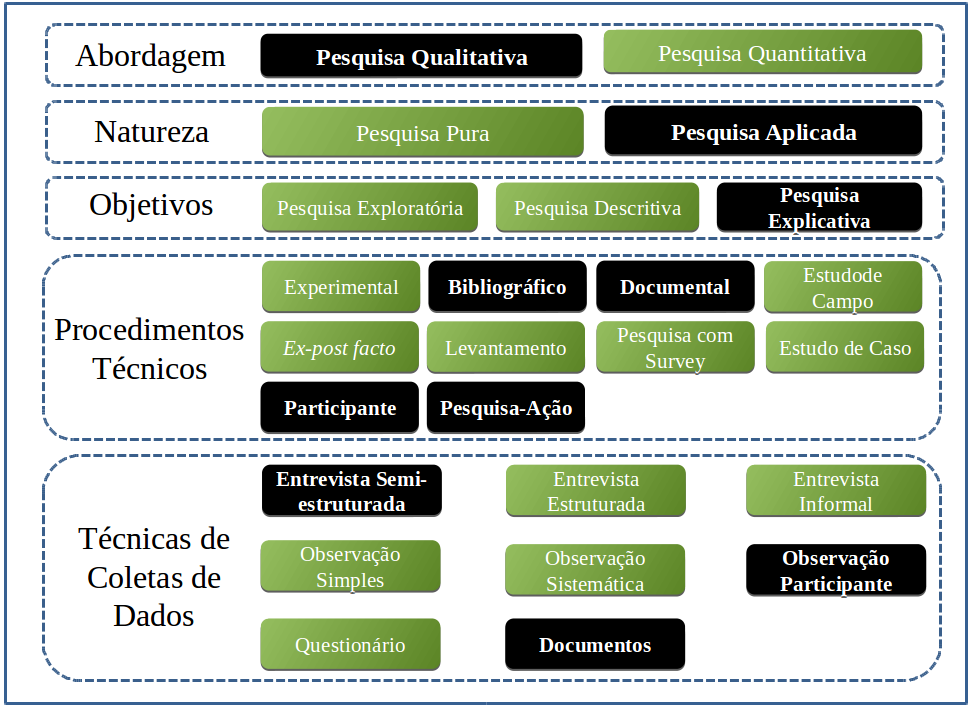
\includegraphics[scale=0.5]{figuras/Metodologia}
	\caption{Seleção da metodologia adotada da pesquisa. Fonte: Autores}
\end{figure}

Nas Subseções seguintes, será dado maior aprofundamento no procedimento, Pesquisa-Ação e na técnica, Entrevista Semi-Estruturada, pois esses serão a base metodológica deste trabalho.

\subsection{Pesquisa-Ação}

Com o grande uso e aumento da sua amplitude e aplicação, a pesquisa-ação tornou-se atualmente um termo aplicado de maneira vaga a qualquer tipo de tentativa de melhora ou de investigação da prática. Assim é necessário que se encare a pesquisa-ação como uma das muitas diferentes formas de investigação-ação a qual é definida como toda tentativa continuada, sistemática e empiricamente fundamentada de aprimorar a prática \cite{tripp2005pesquisa}.

Deve-se reconhecer a pesquisa-ação como um dos inúmeros tipos de investigação-ação, que é um termo genérico para qualquer processo que siga um ciclo no qual se aprimora a prática pela oscilação sistemática entre agir no campo da prática e investigar a respeito dela \cite{tripp2005pesquisa}.

Para Thiollent (2009) no decorrer da pesquisa-ação ocorre um efeito de aprendizagem, por vezes concebido como conscientização. A pesquisa alimenta a ação e vice-versa, sendo que a aprendizagem é difusa ao longo do processo.

Essa metodologia é caracterizada como um método flexível, qualificada pelo constante ciclo das fases. Assim, o processo de execução, geralmente, não é apresentado em ordem cronológica e sim na forma de um conjunto de ações que, embora não ordenadas no tempo, podem ser consideradas como etapas da pesquisa-ação (GIL, 2008; THIOLLENT, 1986).

É necessário que planeja-se, implementa-se, descreva-se e avalie-se uma mudança para a melhora de sua prática, aprendendo mais, no correr do processo, tanto a respeito da prática quanto da própria investigação \cite{tripp2005pesquisa}.

Assim, basicamente essas quatro ações, se constituem nas fases para o processo de pesquisa-ação, como Thiollent (2009) também afirma que a pesquisa-ação tem quatro grandes fases: Fase exploratória, na qual os atores da pesquisa começam a detectar problemas a serem combatidos; Fase de pesquisa, na qual coletam-se dados com diversos instrumentos e a pesquisa é discutida pelos membros; Fase de ação, na qual definem-se objetivos, apresentam-se propostas e resultados; e por fim, a Fase de avaliação, na qual se obtém conhecimento produzido pela pesquisa e analisa os resultados alcançados.

O processo de pesquisa-ação não existe de forma padronizada, pois, dependendo da situação social ou do quadro organizacional em que se aplica, os procedimentos e a ordenação das etapas podem variar. O autor também destaca que as três primeiras fases podem ocorrer simultaneamente Thiollent (2009).

Baseado nessas informações sobre o processo de pesquisa-ação, além das quatro fases básicas previstas, vamos adotar mais uma fase adicional, a fase de coleta de dados, onde é feito o levantamento e coleta dos dados originado das técnicas de coleta de dados e seguir uma adaptação das fases do processo conforme estabelecido por \cite{coughlan2002action}. Dessa forma iremos neste trabalho adotar o seguinte processo de pesquisa-ação para a condução do procedimento:


\begin{figure}[!htb]
	\centering
	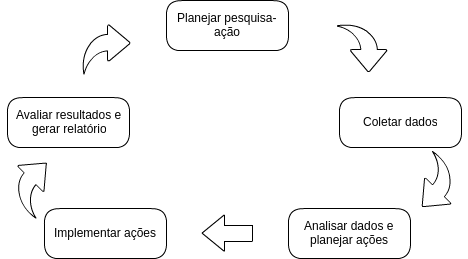
\includegraphics[scale=0.5]{figuras/estruturacao_pesquisa_acao}
	\caption{Estruturação para pesquisa-ação. Fonte: \cite{coughlan2002action}, adaptado}
\end{figure}

\subsection{Entrevista Semi-Estruturada}

------------
--Esse cai fora!!!--
O estudo de caso consiste no estudo profundo e exaustivo de um ou mais objetos, de forma a obter conhecimento amplo e detalhado sobre o mesmo. Segundo \citeonline{yin2001estudo} o estudo de caso é a abordagem mais adequada para a investigação de um fenômeno em seu contexto real, onde os limites entre este fenômeno e o seu contexto não são claramente percebidos. Os propósitos do estudo de caso são \cite{gil2002}:

\begin{itemize}
	\item Explorar situações de contextos reais onde os limites não estão claramente definidos.
	\item Preservar o caráter unitário do objeto.
	\item Descrever a situação do contexto do qual esta sendo feita a investigação.
	\item Desenvolver teorias e formular hipóteses.
	\item Determinar as causas de um determinado fenômeno onde a complexidade não permite o uso de levantamentos e experimentos.
\end{itemize}
--Esse cai fora!!!--
--------------

Existem diversos métodos de coleta de dados para suportar os propósitos de um procedimento técnico, e um dos métodos comumente usados na engenharia de software é a entrevista \cite{caseStudySE}. Quase todos os estudos de caso envolvem algum tipo de entrevista, seja para a finalidade primária de coleta dados, seja para uma validação de outros tipos de dados \cite{caseStudySE}. A entrevista é caracterizada como um método de coleta de dados onde o pesquisador está em contato direto com os entrevistados e como um método de coleta de dados em tempo real \cite{caseStudySE}. O diálogo entre o entrevistador e o entrevistado é guiado por um conjunto de perguntas, que podem ser classificadas como abertas ou fechadas \cite{caseStudySE}. As perguntas abertas permitem uma maior gama de respostas e relatos de problemas, por parte do entrevistado. Já as perguntas fechadas oferecem alternativas mais limitadas, se comparadas as perguntas abertas. Ambos os tipos de perguntas são baseadas nos tópicos de interesse relacionados ao estudo de caso. 

Segundo \cite{caseStudySE}, a entrevista pode ser classificada em três categorias diferentes:
\begin{enumerate}
	\item \textbf{Não-estruturada}: As perguntas são formuladas de forma aberta e de acordo com os interesses do pesquisador. A conversa durante a entrevista irá se desenvolver de acordo com os interesses do entrevistado e do entrevistador.
	\item \textbf{Semiestruturada}: As questões planejadas não são necessariamente perguntadas na ordem em que estão listadas, tendo o desenvolvimento da conversa influência direta na ordem em que as perguntas são feitas ao entrevistado. Além disso, esse tipo de pesquisa permite o improvisamento e a exploração de problemas levantados durante a conversa. É comum em estudos de caso em engenharia de software.
	\item \textbf{Completamente estruturada}: Todas as perguntas são detalhadamente planejadas de antemão e são feitas exatamente na ordem em que estão listadas. Esse tipo de entrevista se assemelha a \textit{surveys} baseados em questionários, pois se trata de perguntas fechadas.
\end{enumerate}

Uma vez que os dados são coletados, o foco se volta para a análise e interpretação dos mesmos. O objetivo desta etapa é derivar conclusões dos dados, buscando a compreensão e a formação de padrões em cima dos mesmos, através de uma cadeia de evidência. Uma cadeia de evidência significa que o leitor pode chegar aos mesmos resultados e conclusões em cima dos dados coletados \cite{caseStudySE}. A análise e interpretação dos dados pode ser dividida nos seguintes procedimentos \cite{caseStudySE}:

\begin{enumerate}
	\item Os dados são codificados de forma que a cada pedaço do texto, que pode ser uma linha ou um parágrafo por exemplo, é atribuído um código que pode representar um certo tema, uma área, uma construção e assim por diante. Observa-se que um pedaço de texto pode possuir mais de um código e um código pode estar associado a mais de um pedaço de texto.
	\item Identificar um conjunto de hipóteses em cima dos dados codificados.
	\item Formar um conjunto de generalizações/conclusões.
	\item Relatar os resultados.
\end{enumerate}


\subsection{Metodologia Adotada}
--essa subseção irá sumir, pois não tem mais sentido falar da metodologia adotada, sendo que na parte da metodologia já está se explicando e informando a metodologia que se irá adotar no trabalho--

A metodologia adotada para este trabalho foi o estudo de caso, devido a necessidade de realizar um diagnóstico da situação atual para a construção da solução de apoio, e o método utilizado no estudo de caso foi a entrevista, por ser um método bastante comum neste tipo de metodologia e permitir um contato direto com os entrevistados. 

A entrevista elaborada pode ser classificada como semiestruturada. No planejamento da entrevista, algumas categorias de perguntas relacionadas ao ciclo de vida do software e ao contexto do desenvolvedor foram elaboradas, de forma a auxiliar na formulação das perguntas.

%TODO: Unificar pesquisa participante junto com a descrição na parte teórica da metodologia, onde é descrito o estudo de caso.
\subsection{Pesquisa Participante}

--Pesquisa participante--
%TODO: Unificar dentro da metodologia também, ou mover esta sub-seção para antes da sub-seção "Metodologia Adotada".

--Essa parte irá sumir, pois ela virou uma técnica adotada chamada observação participante e já foi abordada na metodologia--
\subsection{Fases da Pesquisa}

A partir da metodologia, foram definidas as fases e etapas do trabalho, sendo que as fases forram:

\begin{itemize}
	\item Definição do trabalho,
	\item Pesquisa bibliográfica, 
	\item Pesquisa-ação e documental
	\item Coleta de dados e,
	\item Análise e interpretação
\end{itemize}

Na Figura 3 pode-se observar o plano metodológico adotado para este trabalho e em seguida
uma descrição de cada uma das fases.

\begin{figure}[!htb]
	\centering
	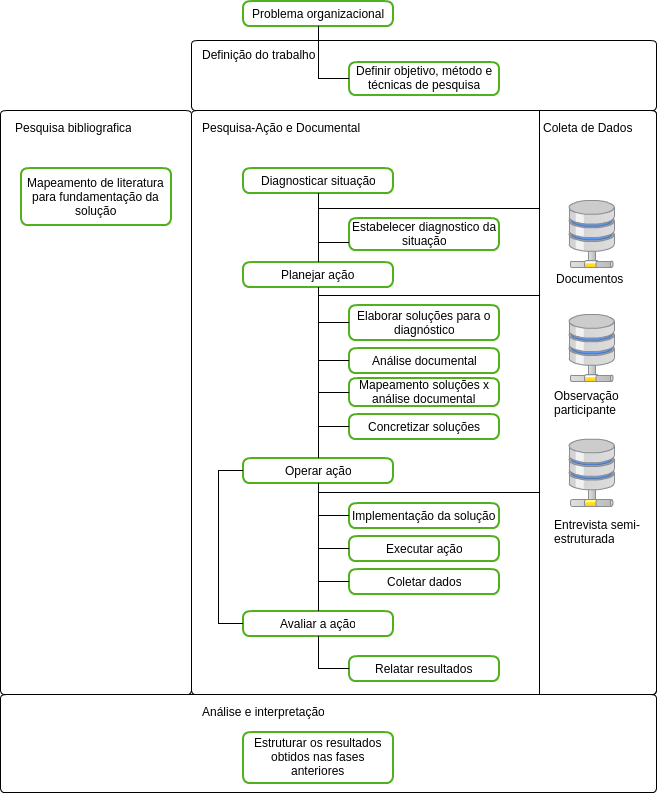
\includegraphics[scale=0.4]{figuras/Plano_metodologico}
	\caption{Plano metodológico adotado. Fonte: autores}
\end{figure}

\textit{Derfinição do Trabalho}

Esta etapa compreende o estabelecimento, com base no problema
organizacional levantado em alto nível: sendo o objetivo a ser atingido, a pergunta de pesquisa, a seleção metodológica e as fases da pesquisa.

\textit{Pesquisa Bibliográfica}

As pesquisas bibliográficas serão realizadas ao longo de toda a pesquisa-ação. Esta fase oferece apoio principalmente para o planejamento da ação, sendo que é nela onde ocorre o mapeamento da literatura para a construção do referencial teórico e definição da ação a ser aplicada.

\textit{Pesquisa-Ação e Documental}

Esta fase é a base do trabalho, onde será realizada as etapas definidas do processo de pesquisa-ação dentro do órgão x, na busca de tentar entender os problemas que ocorrem na prática durante o desenvolvimento de sistemas descentralizados, por meio da experiência de vivência no órgão e pelos documentos inerentes ao mesmo, para enfim surgir com uma solução que apoie esse desenvolvimento.

\textit{Coletas de dados}

Esta fase registra-se os resultados das entrevistas, documentos do órgão e a experiência obtida com o desenvolvimento descentralizado no órgão

\textit{Análise e Interpretação}

Nesta fase os resultados observados nas fases anteriores serão analisados e verificado quanto à solução apoia de forma necessária o desenvolvimento descentralizado do órgão.

\section{\textit{Organização do Trabalho}}

--registrar como está organizado--
--Falar que a partir do capítulo 2 ao 3 (vai entrar mais) trata-se do referencial teórico--

Nos capítulos 2,3 e ... apresenta o referencial que embasa este trabalho. O referencial teórico é o meio em que o autor do trabalho demonstra o seu conhecimento sobre uma determinada área de estudo (teorias, vocabulários, variáveis chave, fenômenos, métodos e história) \cite{randolph2009}.


\chapter[Capítulo 2 - Desenvolvimento descentralizado]{Capítulo 2 - Desenvolvimento descentralizado}

\section{\textit{Considerações Iniciais do Capítulo}}

--Considerações sobre o capítulo--

\section{\textit{End User Development}}

\textit{End User Development} (Desenvolvimento por usuário final) é um modelo de desenvolvimento de software onde o usuário final é o principal responsável pela construção do software. \citeonline{lieberman2006} define o \textit{End User Development} (EUD) como um conjunto de métodos, técnicas e ferramentas que permite aos usuários de sistemas de software, que agem como desenvolvedores de software não profissionais, em algum ponto, criar, modificar ou estender um artefato de software. Dentre as motivações para este modelo de desenvolvimento, destacam-se a diversidade e a mutabilidade dos requisitos, bem como a dificuldade em defini-los em contextos que evoluam com uma alta frequência, o que pode levar o desenvolvimento tradicional a consumir muito tempo e atingir um alto custo \cite{lieberman2006}. Além disso, uma organização que possui uma demanda por informatização dos seus processos de trabalho, por parte das suas diferentes áreas de negócio, superior a capacidade produtiva da área de TI, pode não conseguir atender certas áreas por conta das priorizações das demandas \cite{artigoTcuGovTI}. O EUD acelera as respostas às mudanças e contorna o problema de definição dos requisitos, porque os usuários finais geralmente são especialistas no domínio em que estão inseridos, ou seja, são os detentores dos requisitos da solução computacional \cite{fischer2004}. O fato de cada usuário final ser um potencial desenvolvedor também contribui para um aumento da capacidade produtiva da TI.

Para que o desenvolvimento seguindo este modelo possa ocorrer é necessário que existam meios para que o usuário final possa desenvolver e adaptar o software, e para tanto a tecnologia envolvida deve diminuir o esforço cognitivo necessário para a construção do software, através da aproximação conceitual entre as ações do mundo real e as do mundo da programação \cite{fischer2004}. Os usuários finais geralmente não possuem habilidades de um profissional da área de software, e também não estão interessados em construir sistemas no mesmo nível que esses profissionais, por isso é necessário que a tecnologia usada no desenvolvimento alinhe a complexidade relacionada a esta atividade com as habilidades do usuário final. A motivação dos usuários finais é algo essencial para o favorecimento deste modelo, e fatores como o empoderamento, a velocidade de desenvolvimento, a flexibilidade e o controle influenciam diretamente na motivação desses usuários.

O principal objetivo do EUD é oferecer meios para que os usuários finais consigam desenvolver e adaptar software \cite{lieberman2006}. Desta maneira, as aplicações preparadas para o EUD devem ser, principalmente, flexíveis, fáceis de se entender, de se usar, e de se ensinar \cite{lieberman2006}. A preocupação com a tecnologia usada neste modelo de desenvolvimento, mais especificamente na parte das linguagens de programação e aplicações de desenvolvimento, é a relação escopo de aplicação versus esforço de aprendizagem. A figura 1 ilustra a relação do escopo de aplicação e do custo de aprendizagem, para diferentes linguagens de programação e aplicações. Linguagens de programação mais tradicionais como C++ e JAVA oferecem a possibilidade de construção de software de uma grande variedade de domínios, porém a um alto custo associado ao esforço de aprendizagem. Outras linguagens possuem um menor esforço de aprendizagem, ao custo de uma limitação no escopo de aplicação. As linguagens ou aplicações de desenvolvimento ideais para o EUD são as que possuem um alto escopo de aplicação e um baixo esforço de aprendizagem \cite{fischer2004}. As que existem atualmente só utilizam uma pequena parte do potencial do EUD, com algumas falhas \cite{paterno2013}.

\begin{figure}[h]
	\centering
	\label{fig01}
		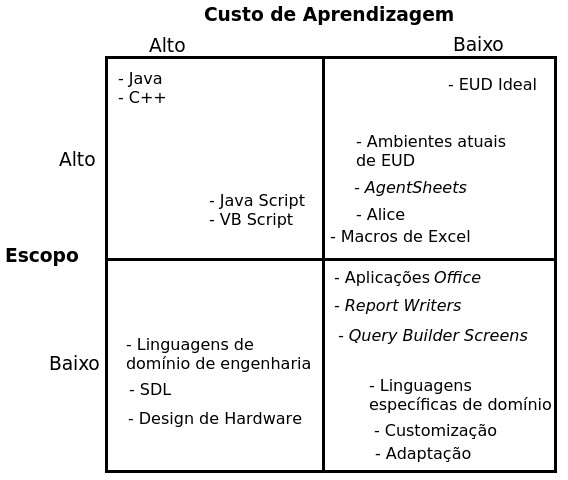
\includegraphics[scale=0.8]{figuras/trade_off_eud_editado}
	\caption{Relação escopo de aplicação e custo de aprendizagem}
\end{figure}
\pagebreak

\citeonline{lieberman2006} classifica as atividades do usuário final em dois tipos:

\begin{enumerate}
\item \textbf{Parametrização ou Customização:} São atividades que permitem o usuário escolher comportamentos, apresentações e mecanismos  alternativos, que já existem dentro de uma aplicação.

\item \textbf{Criação e modificação de programas:} São atividades que implicam na criação ou modificação de artefatos de software. Macros e linguagens de \textit{script} são exemplos deste tipo de atividade.
\end{enumerate}

\section{Desenvolvimento descentralizado}

O desenvolvimento descentralizado é uma adaptação do modelo EUD ao serviço público federal brasileiro. A diferença entre o EUD e o desenvolvimento descentralizado é que no desenvolvimento descentralizado não é necessariamente o usuário final do software quem irá desenvolve-lo \cite{artigoTcuGovTI}. No Órgão X, que foi um dos pioneiros na implantação deste modelo, os projetos que seguem o desenvolvimento descentralizado tem sido desenvolvidos, na maioria das vezes, por estagiários de TI, que possuem diferentes níveis de conhecimento sobre desenvolvimento de software, e que também não são os usuários finais do software \cite{artigoTcuGovTI}. O desenvolvedor, se for um estagiário, é alocado na área de negócio e um analista de TI é designado para dar suporte técnico a área de negócio, de forma a garantir que o software sendo desenvolvido siga os padrões estabelecidos e garantidos pela TI corporativa \cite{artigoTcuGovTI}.
Dentre as possíveis motivações que tem levado a adoção deste modelo em alguns órgãos da administração pública federal, destacam-se \cite{slideTCU}:

\begin{itemize}
\item Desconhecimento das iniciativas de informatização;
\item Falta de alinhamento estratégico das iniciativas;
\item Duplicidade de esforços das unidades de negócio;
\item Diversidade de ferramentas de desenvolvimento;
\item Elevado risco de descontinuidade;
\item Comprometimento da segurança da informação;
\end{itemize}
\clearpage

\section{Oracle Application Express - APEX}

O Oracle Application Express (APEX) é uma ferramenta que permite criar, personalizar e implementar aplicações em cima do banco de dados Oracle, usando apenas um navegador de internet. O APEX é um ambiente de desenvolvimento gratuito para construir aplicações usando SQL e PL/SQL e que apresenta uma plataforma extensível, executada dentro do banco de dados Oracle \cite{oracleApex}. O APEX tem como objetivo diminuir a complexidade de desenvolvimento das aplicações, ao fornecer um ambiente interativo e de fácil manuseio para construir e executar as aplicações, garantindo que tanto desenvolvedores não profissionais quanto desenvolvedores experientes desenvolvam com agilidade. As funcionalidades da aplicação são criadas de forma fácil e rápida. As vantagens do APEX incluem \cite{oracleApex}:
\begin{itemize}
\item Velocidade de entrega;
\item Maior controle e precisão no desenvolvimento;
\item Facilidade para a criação de protótipos;
\item Facilidade de implantação;
\item Aplicação acessada via navegador (URL);
\item Grande quantidade de usuários (desenvolvedores) ativos;
\end{itemize}

Além disso, o ambiente de desenvolvimento integrado é muito intuitivo, o que torna a introdução e a adoção do APEX uma transição fácil para desenvolvedores experientes ou usuários finais.

O APEX usa uma arquitetura simples, onde as páginas são geradas dinamicamente usando metadados armazenados no banco de dados Oracle. Não há geração de código ou compilação de arquivos. Uma vez que ele foi instalado e configurado, a URL será a via de acesso ao ambiente de desenvolvimento e às aplicações, tanto para os desenvolvedores quanto para os usuários finais. As alterações feitas durante o desenvolvimento são salvas diretamente nas tabelas de metadados, que contém as definições das aplicações. Após isso o desenvolvedor pode executar a aplicação e revisar as melhorias imediatamente.
Para a implantação e execução do APEX é necessário um servidor web, um servidor de aplicação, um servidor APEX \textit{listener} e um servidor de banco de dados Oracle, conforme a figura 2.
\clearpage

\begin{figure}[!htb]
	\centering
		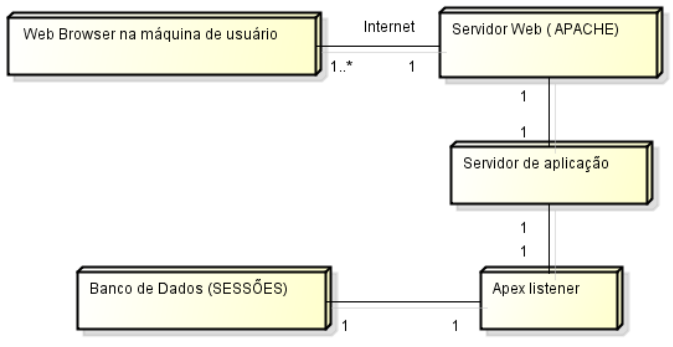
\includegraphics[scale=0.6]{figuras/arquitetura_apex}
	\caption{Arquitetura do APEX \cite{ferreira2015}.}
\end{figure}

O fluxo de dados na arquitetura do APEX, é composto dos seguintes passos \cite{ferreira2015}:
\begin{enumerate}
\item Uma requisição HTTP é enviada, pelo navegador, quando o usuário acessa uma página da aplicação;
\item O servidor web recebe a requisição e identifica que é uma requisição do APEX, redirecionando a requisição ao servidor de aplicação correto;
\item O servidor de aplicação organiza os pedidos (filtros, \textit{cache}, \textit{timeouts}, filas, etc) e transfere para o APEX \textit{listener}.
\item O APEX \textit{listener} recebe o pedido e executa os comandos Java que irão ler os dados do banco e/ou executar códigos PL/SQL. O APEX \textit{listener} interage com sessões de banco, onde os dados são buscados.
\item Faz-se o caminho inverso com os dados coletados, os PL/SQLs executados e os códigos HTML, \textit{Javascript}, CSS, \textit{Ajax} e \textit{jQuery} gerados, que são devolvidos ao navegador que então mostra a tela da aplicação ao usuário.
\end{enumerate} 

\chapter[Capítulo 3 - Metodologia ágil]{Metodologia ágil}

A metodologia ágil é uma abordagem de desenvolvimento de software que tem ganhado visibilidade ao longo dos últimos anos, e surgiu através do estabelecimento, entre vários desenvolvedores experientes, de um senso comum de valores no desenvolvimento de software. Um grupo de 17 desenvolvedores, com grande experiência nos mais variados ramos da indústria de software, se reuniu em \textit{Utah} nos Estados Unidos por volta de 2001 para racionalizar uma filosofia comum sobre o que consideravam que tinha valor no desenvolvimento de software. A essa filosofia comum entre os participantes deram o nome de \textit{agile} (ágil) \cite{metodoAgil}. Com base nas experiências de sucesso e fracasso em projetos de software por parte desse grupo, entrando em um acordo comum sobre o que funcionou e o que não funcionou, foi elaborado o Manifesto Ágil para o Desenvolvimento de Software, que norteia os valores e princípios da metodologia ágil \cite{metodoAgil}. O Manifesto Ágil tem como valores \cite{metodoAgil}:

\begin{itemize}
\item Indivíduos e interações ao invés de processos e ferramentas;
\item Software funcionando ao invés de documentação extensiva;
\item Colaboração do cliente ao invés de negociação de contratos;
\item Responder às mudanças ao invés de seguir um plano;
\end{itemize}

Existem vários métodos dentro da metodologia ágil, entre eles: \textit{Extreme Programming} (XP), \textit{Scrum}, \textit{Feature Driven Development} (FDD), \textit{Crystal}, \textit{Lean Development} e etc \cite{agileMethods}.

\section{\textit{Scrum}}

O \textit{Scrum} é um método de gerência de projetos de software que faz parte da metodologia ágil de desenvolvimento de software e que tem atraído cada vez mais atenção ao longo dos últimos anos. O \textit{Scrum} parte da premissa de que o desenvolvimento de software é muito complexo e imprevisível para ser precisamente planejado de início, e por isso um processo de controle mais empírico deve ser aplicado, objetivando garantir visibilidade, inspeção e adaptação \cite{scrum2005}. Visibilidade significa dar a noção de progresso do projeto com a entrega frequente de incrementos de software executável. Inspeção significa que todos do time devem inspecionar os produtos de trabalho gerados por todos, visando a detecção de erros e o estabelecimento de um senso comum sobre o progresso do projeto. Adaptação significa aceitar as mudanças, já que o desenvolvimento de software é uma atividade complexa e imprevisível \cite{agile2014}. As diferentes variáveis técnicas envolvidas em um projeto de software, como prazo, qualidade, requisitos, recursos, tecnologias de implementação e ferramentas,  devem ser controladas constantemente através de um processo iterativo e incremental \cite{scrum2005}.

Existem 3 papéis envolvidos no \textit{Scrum}, o \textit{Product Owner}, o Time, e o \textit{Scrum Master}, e eles são descritos da seguinte forma \cite{scrum2005}:

\begin{itemize}
\item \textbf{\textit{Product Owner}}: Responsável por representar os interesses dos \textit{stakeholders} no projeto, através do suporte de negócio ao time de desenvolvimento. O \textit{Product Owner} também é responsável por manter o \textit{Product Backlog} (\textit{Backlog} do Produto), que é uma lista priorizada de requisitos que irão se tornar uma funcionalidade no software.

\item \textbf{Time}: Responsável por desenvolver a funcionalidade, o time é quem de fato irá transformar uma parte do \textit{Backlog} do Produto em um incremento de funcionalidade ao final de uma iteração. O time deve ser auto-gerenciável, auto-organizável e multi-funcional.

\item \textbf{\textit{Scrum Master}}: Responsável por gerenciar o processo \textit{Scrum}, garantindo que a implementação do \textit{Scrum} se adeque a cultura da organização e que ao mesmo tempo traga os benefícios esperados. Além disso, o \textit{Scrum Master} também deve garantir o esclarecimento do \textit{Scrum} a todos do time e que todos sigam as regras e práticas do \textit{Scrum}.
\end{itemize}

As figuras 3 e 4 mostram, respectivamente, uma visão geral e detalhada do \textit{Scrum}.

\begin{figure}[!htb]
	\centering
		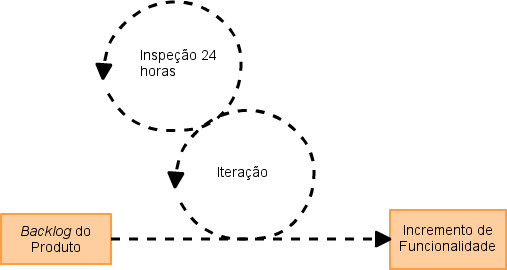
\includegraphics[scale=0.7]{figuras/scrum}
	\caption{Visão geral do \textit{Scrum} \cite{scrum2005}.}
\end{figure}

\begin{figure}[!htb]
	\centering
		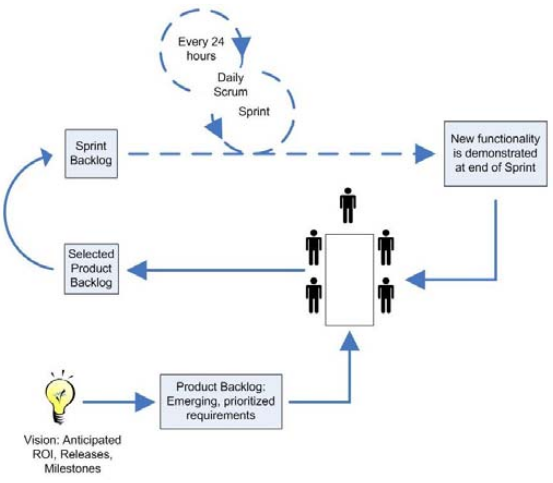
\includegraphics[scale=0.8]{figuras/scrum_detalhado}
	\caption{Visão detalhada do \textit{Scrum} \cite{scrum2005}.}
\end{figure}
\clearpage

Um projeto seguindo o \textit{Scrum} começa com uma visão do sistema a ser desenvolvido, e a partir desta visão o \textit{Backlog} do Produto é definido e priorizado, de acordo com os requisitos conhecidos até então. Uma iteração é chamada de \textit{Sprint}, que geralmente possui a duração de no máximo 1 mês. O trabalho a ser realizado em uma \textit{Sprint} é definido na reunião de planejamento da \textit{Sprint}, onde o \textit{Product Owner} e o time colaboram para estabelecer o que deve ser feito: o \textit{Product Owner} diz ao time o que do \textit{Backlog} do Produto é desejado para a \textit{Sprint}, e o time diz ao mesmo o que acredita que deva ser cumprido ao final da \textit{Sprint}. Ao fim da reunião o \textit{Backlog} da \textit{Sprint} é definido, que é uma lista de tarefas a serem feitas na \textit{Sprint}, onde cada uma deve levar entre 4 a 16 horas para ser finalizada. Ao serem finalizadas, essas tarefas irão entregar um incremento de funcionalidade ao produto. Durante a execução da \textit{Sprint}, reuniões diárias de 15 minutos chamadas de \textit{Daily Scrum Meeting} acontecem. Nestas reuniões, cada membro do time deve responder três questões, objetivando o alinhamento de todos os membros: o que você fez no projeto desde de a última reunião? O que você irá fazer até a próxima reunião? Você tem algum obstáculo em relação aos seus objetivos? Ao final de cada \textit{Sprint}, uma revisão de \textit{Sprint} é realizada, onde o time apresenta ao \textit{Product Owner} e a outros interessados que participam da reunião, o que foi desenvolvido. Ao final da revisão de \textit{Sprint} e antes da próxima reunião de planejamento da \textit{Sprint}, é feita uma retrospectiva, listando os pontos fortes e fracos da \textit{Sprint}, objetivando a melhoria constante. O planejamento da \textit{Sprint}, o \textit{Daily Scrum Meeting}, a revisão de \textit{Sprint} e a retrospectiva são os métodos usados pelo \textit{Scrum} para constituir o controle empírico do desenvolvimento de software \cite{scrum2005}.

\section{Quadro \textit{kanban}}

O método \textit{Kanban} é um termo que surgiu no Japão com o sistema de produção da Toyota para o controle da fabricação de automóveis, onde a demanda é quem dita o ritmo de produção, sinalizando quando é necessário aumentar o mesmo. Desta forma, a indústria adapta a sua velocidade de produção de acordo com o nível de consumo dos clientes. O \textit{Kanban} é um termo japonês que significa sinal visual, portanto uma de suas grandes características é evidênciar os problemas existentes no processo \cite{silva2010kanban}.

Na indústria de software, o uso do método \textit{Kanban} tem ganhado significativo aumento desde de 2007, quando ele foi publicado nas conferências "Lean New Product Development" e "Agile 2007", por Rick Garber e David J. Anderson. Ele é um método pouco prescritivo e bastante adaptativo, por conta disso ele acaba se tornando um método quase que exclusivamente empírico, seguindo apenas três premissas \cite{silva2010kanban}:

\begin{itemize}
\item Visualizar o fluxo de trabalho atual;
\item Limitar o fluxo de trabalho;
\item Acompanhar e gerênciar o fluxo de trabalho;
\end{itemize}

Para dar a noção visual de continuidade do fluxo de trabalho, o método \textit{Kanban} se utiliza do quadro \textit{kanban}. No desenvolvimento de software, o quadro \textit{kanban} é uma ferramenta que permite aos times visualizarem o seu fluxo de trabalho, e ele consiste de colunas desenhadas em um quadro branco com adesivos ou bilhetes colados em cada coluna. Tipicamente ele é composto por 3 colunas: \textit{To Do} (O que fazer), \textit{In Progress} (Em progresso) e \textit{Done} (Concluído) \cite{agile2014}. Cada uma dessas colunas são compostas por tarefas, que precisam ser concluídas para se atingir um determinado objetivo. No caso da metodologia \textit{Scrum}, estas tarefas são geralmente derivadas do \textit{backlog} do produto. Observa-se que pelo fato de o método \textit{Kanban} ser empírico, o quadro \textit{kanban} também acaba se tornando, podendo haver variações nas colunas que o compõe de acordo com as necessidades do time de desenvolvimento \cite{agile2014}. A figura 5 mostra um esquemático de um quadro \textit{kanban}.

\begin{figure}[!htb]
	\centering
		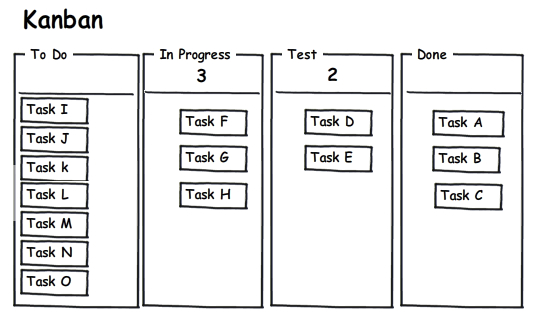
\includegraphics{figuras/Kanban}
	\caption{Esquemático de um quadro \textit{kanban} \cite{kanbanImage}.}
\end{figure}

\chapter[Capítulo 4 – Proposta do Trabalho]{Capítulo 4 – Proposta do Trabalho}

\section{\textit{Considerações Iniciais do Capítulo}}

--falar sobre considerações iniciais--

\section{\textit{Definição da Proposta}}

O presente trabalho está inserido no contexto do Órgão X, onde o Órgão X possui duas formas distintas de desenvolvimento de software: uma forma corporativa, que é uma forma tradicional de desenvolvimento de software (desenvolvimento realizado na área da TI e por profissionais de TI), e uma forma descentralizada, que é uma forma menos tradicional de desenvolvimento (desenvolvimento realizado nas áreas de negócio e por pessoas com menos qualificação técnica e experiência, geralmente estagiários).
O desenvolvimento descentralizado apresenta um bom relato de satisfação no Órgão X, porém alguns problemas de qualidade e manutenibilidade das aplicações tem sido recorrentes.

Tendo em vista esse contexto, este trabalho se propõe a elaborar uma solução informatizada que possa apoiar o desenvolvimento descentralizado no Órgão X, onde esta solução irá conter um conjunto de atividades, de boas práticas e de funcionalidades, que possam contribuir para uma melhoria na qualidade e manutenibilidade das aplicações desenvolvidas. O escopo deste trabalho se limita a desenvolver o conjunto de atividades e boas práticas da solução, de forma que estas atividades estejam relacionadas entre si através de um fluxograma, e que as boas práticas estejam contidas dentro das atividades, auxiliando a execução das mesmas. No próximo trabalho, espera-se detalhar as atividades e as boas práticas definidas, informatizar o fluxo de atividades, e implementar as funcionalidades que possam auxiliar na execução de algumas das atividades da solução.

Para se atingir o objetivo deste trabalho, realizou-se, inicialmente, um levantamento bibliográfico sobre os tópicos relacionados ao trabalho: \textit{End User Development}, desenvolvimento descentralizado, \textit{SCRUM} e \textit{Kanban}. Em seguida foram realizadas entrevistas com o propósito de diagnosticar a situação do desenvolvimento descentralizado no Órgão X, coletando os problemas, as boas práticas e as sugestões de melhorias, relatados pelos próprios desenvolvedores. Foi realizada uma análise em um processo de desenvolvimento descentralizado não implementado, existente no Órgão X, com o intuito de verificar quais atividades e guias existentes, que poderiam dar um suporte à elaboração das soluções relacionadas ao diagnóstico obtido. Uma análise sobre os conteúdos da \textit{Wiki} da unidade coordenadora do desenvolvimento descentralizado também foi feita, de forma a agregar algumas boas práticas, definidas pela unidade, à solução. A partir do diagnóstico, da análise do processo e da análise da \textit{Wiki} foram definidas as atividades e os guias da solução de apoio. Estas atividades foram então relacionadas através de um fluxograma, representando o sequenciamento das mesmas.

%TODO: Explicar aqui a elaboração da entrevista, já que a entrevista é um "método" da pesquisa participante.
\begin{comment}
\section{\textit{Pesquisa Participante}}
--Falar como a gente abordou a pesquisa participante--
\end{comment}

\section{Entrevista Realizada}
A entrevista teve como objetivo realizar um diagnóstico da situação do desenvolvimento descentralizado no Órgão X, sob o ponto de vista do desenvolvedor que esta inserido neste contexto. Esse diagnóstico procurou abordar os aspectos de problemas, de boas práticas realizadas e de sugestões de melhorias. Para que esses aspectos pudessem ser abordados na entrevista, dividiu-se a mesma em categorias, onde estas categorias estão, em sua maioria, relacionadas as fases de um ciclo de desenvolvimento de software. Cada categoria possui um objetivo, que representa qual o tipo de informação que se pretende obter. Na tabela 1 estão expostas as informações desejadas, através dos objetivos, e suas respectivas categorias.

\begin{comment}
O objetivo da entrevista consistiu em obter um diagnóstico da situação atual do desenvolvimento descentralizado no Órgão X, para que servisse de insumo para a elaboração da solução de apoio. Como diagnóstico entendeu-se as boas práticas realizadas, as sugestões de melhoria e os problemas. Portanto, a entrevista elaborada tentou abordar esses pontos, consistindo de 34 perguntas divididas em 9 categorias. A entrevista pode ser visualizada no "Anexo A".
\end{comment}

\begin{table}[!htb]
\centering
\caption{Categorias da entrevista e seus objetivos.}
\begin{tabular}{|l|l|}
\hline
\textbf{Categoria}                                                   & \textbf{Objetivo}                                                                                                                                                                                                                                                                                                                            \\ \hline
\begin{tabular}[c]{@{}l@{}}Descrição do\\ Desenvolvedor\end{tabular} & 1- Obter informações sobre o perfil dos desenvolvedores.                                                                                                                                                                                                                                                                                     \\ \hline
\begin{tabular}[c]{@{}l@{}}Papel do\\ Desenvolvedor\end{tabular}     & 1- Obter informações sobre o papel do desenvolvedor no órgão.                                                                                                                                                                                                                                                                                \\ \hline
\begin{tabular}[c]{@{}l@{}}Efetividade do\\ Curso\end{tabular}       & 1- Obter informações sobre a preparação dos novos desenvolvedores.                                                                                                                                                                                                                                                                           \\ \hline
Requisitos                                                           & \begin{tabular}[c]{@{}l@{}}1- Obter informações sobre como se dá o levantamento de requisitos \\ nos departamentos da instituição.\\ 2- Obter informações de como é armazenado e gerenciado os requisitos \\ do sistema a ser desenvolvido.\\ 3- Obter informações de como é englobado as mudanças de requisitos \\ ao sistema.\end{tabular} \\ \hline
\textit{Design}                                                      & \begin{tabular}[c]{@{}l@{}}1- Obter informações sobre como é realizado a modelagem (arquitetura) \\ do sistema.\end{tabular}                                                                                                                                                                                                                 \\ \hline
Codificação                                                          & \begin{tabular}[c]{@{}l@{}}1- Obter informações sobre a depuração de erros do sistema.\\ 2- Obter informações sobre estilos de codificação.\\ 3- Obter informações sobre o ambiente de codificação.\end{tabular}                                                                                                                             \\ \hline
Teste                                                                & \begin{tabular}[c]{@{}l@{}}1- Obter informações sobre a realização dos testes, bem como a forma \\ de realizá-los.\end{tabular}                                                                                                                                                                                                              \\ \hline
Implantação                                                          & 1- Obter informações sobre a migração, para a produção, do sistema.                                                                                                                                                                                                                                                                          \\ \hline
\end{tabular}
\end{table}

A categoria "Descrição do Desenvolvedor" serviu unicamente para descrever o perfil dos desenvolvedores entrevistados, portanto ela não foi considerada na análise dos resultados obtidos. A partir dessas categorias, foram elaboradas as perguntas, de forma que elas atendessem os objetivos definidos. O \textit{template} da entrevista pode ser visualizo no "Anexo A".

Uma vez que a entrevista foi elaborada, o próximo passo consistiu em aplicá-la. A escolha dos desenvolvedores foi feita de forma aleatória, escolhendo-se 8 desenvolvedores diferentes que estão inseridos no contexto do desenvolvimento descentralizado do Órgão X. Os 8 desenvolvedores escolhidos estão divididos entre 7 estagiários e 1 servidor. A tabela 2 contextualiza o perfil dos desenvolvedores entrevistados. Observa-se que alguns desses dados não se aplicam ao desenvolvedor 6, por este ser um servidor.

\newcolumntype{M}[1]{>{\centering\arraybackslash}m{#1}}
\begin{table}[!htb]
	\centering
	\caption{Perfil dos desenvolvedores entrevistados}
	\begin{tabular}{|M{2.88cm} | M{2.8cm} | M{2.2cm}| M{2.8cm} | M{2.2cm}|}
		\hline
		\textbf{Desenvolvedor} & \textbf{Unidade} & \textbf{Tempo de estágio} & 
		\textbf{Curso} & \textbf{Tempo de Curso} \\ \hline
		Desenvolvedor 1 & SECOM & 1 ano & Análise e Desenvolvimento de Sistemas & 2 semestres \\
		\hline
		Desenvolvedor 2 & SCV & 1 ano & Sistemas de Informação & 8 semestres \\
		\hline
		Desenvolvedor 3 & MTCU & 7 meses & Sistemas de informação & 6 semestres \\
		\hline
		Desenvolvedor 4 & SEADE & 7 meses & Análise e Desenvolvimento de Sistemas & 4 semestres \\
		\hline
		Desenvolvedor 5 & SECOF & 1 ano & Sistemas de Informação & 5 semestres \\
		\hline
		Desenvolvedor 6 & SEPROD & - & - & - \\
		\hline
		Desenvolvedor 7 & DISIC & 1 mês & Engenharia de Software & 6 semestres \\
		\hline
		Desenvolvedor 8 & SEPROD & 6 meses & Engenharia de Redes de Comunicação & 9 semestres \\
		\hline
	\end{tabular}
	\label{tab02}
\end{table}

Após a aplicação da entrevista, o foco voltou-se a análise dos dados da mesma. A análise feita consistiu dos seguintes passos:

\begin{comment}
\begin{enumerate}
	\item Atribuir um código, previamente estabelecido, a uma unidade de resposta, que pode ser uma frase ou um conjunto de frases que tratem de um mesmo assunto.
	\item Agrupar as unidades de resposta de acordo com as categorias de código que receberam.
	\item Dentro de uma categoria de código, agrupar as unidades de respostas semelhantes.
	\item Elaborar ações para as unidades de respostas agrupadas dentro das categorias de códigos.
\end{enumerate}
\end{comment}

\begin{enumerate}
	\item Atribui-se um código, previamente estabelecido, a uma unidade de resposta, que pode ser uma frase ou um conjunto de frases que tratem de um mesmo assunto.
	\item Agrupou-se as unidades de resposta de acordo com as categorias de código que receberam.
	\item Dentro de uma categoria de código, rotulou-se as respostas com o uso de chaves, que representam o sentido específico de uma resposta.
	\item Agrupou-se todas as chaves únicas obtidas, de forma a construir um conjunto de chaves únicas.
	\item Elaborou-se ações para as chaves dentro do conjunto.
\end{enumerate}

Os códigos foram derivados dos objetivos de cada categoria de perguntas do ciclo de vida. A Tabela \ref{tab01} ilustra os códigos derivados de cada objetivo definido.

\newcolumntype{M}[1]{>{\centering\arraybackslash}m{#1}}
\begin{table}[!htb]
	\centering
	\caption{Códigos elaborados para a análise dos resultados}
	\begin{tabular}{|M{4.8cm} | M{4.8cm} | M{4.8cm}|}
		\hline
		\textbf{Categoria} & \textbf{Objetivo} & 
		\textbf{Código Derivado} \\ \hline
		Descrição do desenvolvedor & Obter informações sobre o perfil dos desenvolvedores & 
		Perfil do Desenvolvedor \\ \hline
		Papel do desenvolvedor & Obter informações sobre o papel do desenvolvedor no órgão & 
		Papel do Desenvolvedor \\ \hline 
		Efetividade do curso & Obter informações sobre a preparação dos novos desenvolvedores & 
		Preparação \\ \hline 
		Requisitos & Obter informações sobre como se dá o levantamento de requisitos nos departamentos da instituição & Elicitação de Requisitos \\ \cline{2-3}
		& Obter informações de como é armazenado e gerenciado os requisitos do sistema a ser desenvolvido &
		Gerenciamento de Requisitos \\ \cline{2-2}
		& Obter informações de como é englobado as mudanças de requisitos ao sistema & \\ \hline
		\textit{Design} & Obter informações sobre como é realizado a modelagem (arquitetura) do sistema &
		Modelagem do sistema \\ \hline
		Codificação & Obter informações sobre a depuração de erros do sistema & Depuração \\ \cline{2-3}
		& Obter informações sobre estilos de codificação & Estilos de codificação \\ \cline{2-3}
		& Obter informações sobre o ambiente de codificação & Ambiente de codificação \\ \hline
		Teste & Obter informações sobre a realização dos testes, bem como a forma de realiza-los &
		Teste \\ \hline
		Implantação & Obter informações sobre a migração, para a produção, do sistema & Implantação \\
		\hline
	\end{tabular}
	\label{tab01}
\end{table}

As chaves foram derivadas dos significados das respostas das entrevistas, de forma que se duas ou mais respostas geraram uma mesma chave, devido aos seus significados semelhantes, somente uma única chave foi considerada. A figura 2 mostra um esquemático que exemplifica a execução dos passos definidos para a análise.

%TODO: Inserir a figura aqui talvez.
\begin{figure}[h]
	\centering
	\label{fig02}
		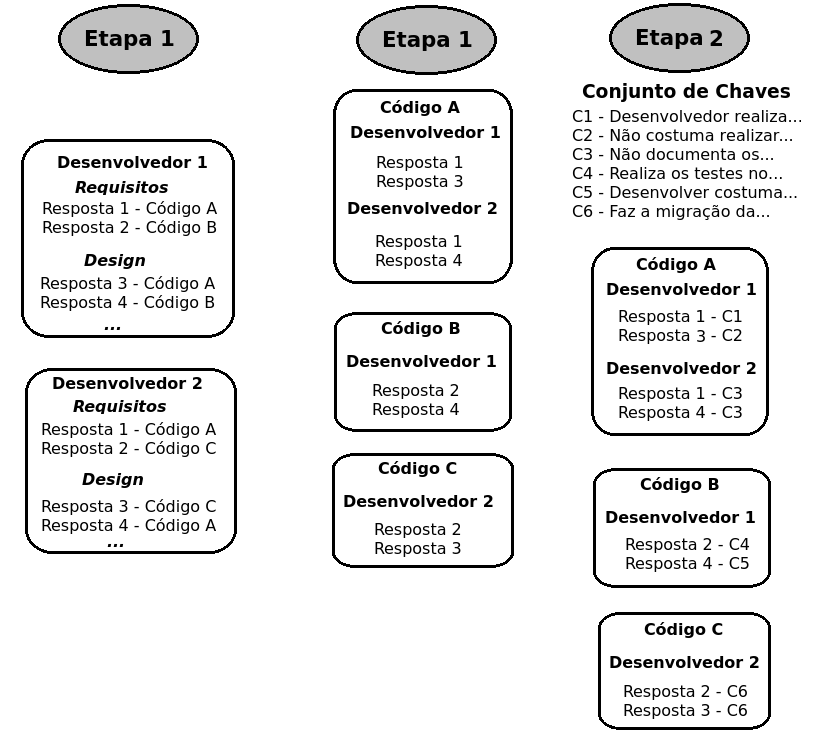
\includegraphics[scale=0.7]{figuras/Esquematico_Analise_2}
	\caption{Etapas realizadas na análise das respostas.}
\end{figure}

A atribuição de um código e de uma chave foram necessários, pois dentro de um determinado assunto, representado pelo código, ainda poderiam haver respostas semelhantes. Desta forma, garante-se que o conjunto final de chaves conterá somente chaves únicas, ou seja, respostas únicas, eliminando a redundância no diagnóstico.
\clearpage

\section{Processo de Desenvolvimento Descentralizado}

A necessidade de um processo ou guia para o desenvolvimento descentralizado é algo já foi percebido pelo Órgão X, pois uma tentativa de implantação de um processo já havia sido realizada. O processo, chamado de Processo de Desenvolvimento Descentralizado do Órgão X, teve a sua finalização concluída no ano de 2012, e foi elaborado pela Secretaria de Tecnologia da Informação do órgão. Apesar de o processo ter sido desenvolvido, segundo o chefe da unidade coordenadora do desenvolvimento descentralizado, ele nunca chegou ao conhecimento dos desenvolvedores devido a questões normativas do próprio órgão, que inviabilizaram a sua implantação (CITAR O DEPOIMENTO???).

O processo, elaborado na ferramenta \textit{Eclipse Process Framework}, que é voltada à construção de processos, consiste de 6 fases bem definidas: Estudo Preliminar de Projeto, Elicitação de Requisitos, Projeto de Banco de Dados, Construção, Homologação e Implantação. Cada uma dessas fases são divididas em atividades e tarefas, que por sua vez são apoiadas por um conjunto de guias e modelos.

\begin{figure}[h]
	\centering
		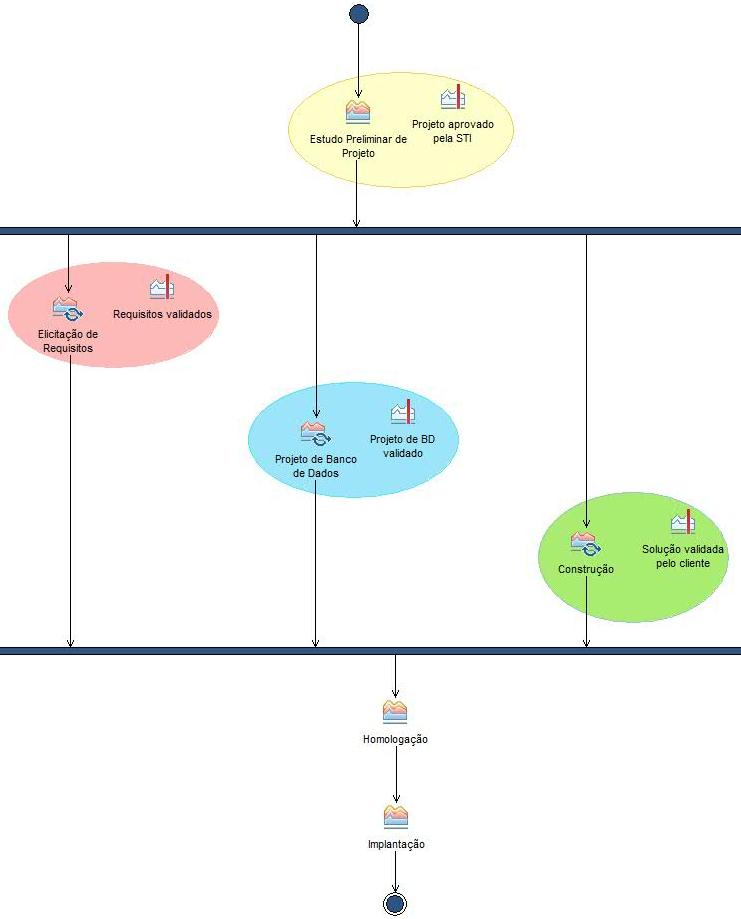
\includegraphics[scale=0.8]{figuras/PDESC}
	\caption{Ciclo de vida do processo de desenvolvimento descentralizado.}
\end{figure}

\begin{enumerate}
	\item \textbf{Estudo Preliminar de Projeto:} Fase destinada à análise da proposta de solução e, caso a proposta seja aprovada, à preparação de recursos.
	\item \textbf{Elicitação de Requisitos:} Fase destinada à elicitação de requisitos e à definição da arquitetura da solução.
	\item \textbf{Projeto de Banco de Dados:} Fase destinada à construção do Modelo de Dados Lógico e do Modelo de Dados Físico da solução.
	\item \textbf{Construção:} Fase destinada á construção da solução.
	\item \textbf{Homologação:} Fase destinada à realização dos testes da solução, à capacitação dos usuários e à divulgação da solução.
	\item \textbf{Implantação:} Fase destinada à implantação da solução.
\end{enumerate}
\clearpage

Foram selecionados, para a construção da solução de apoio, os componentes de processo (atividades, tarefas, guias e modelos) que possuem uma relação com os problemas, as sugestões e as boas práticas, relatados no diagnóstico, e alguns que não estão relacionados diretamente com o diagnóstico mas que julgou-se interessante para complementar a solução.

\section{\textit{Wiki} do Desenvolvimento Descentralizado}

O Órgão X utiliza um sistema de \textit{Wiki} como uma das formas de compartilhamento de informação entre o público interno do órgão, de forma que esse público possa usufruir e contribuir com as informações publicadas. A unidade coordenadora do desenvolvimento descentralizado também possui a sua página dentro da \textit{Wiki}, onde são definidos os guias e as boas práticas, que contribuam para uma melhoria na qualidade das aplicações e que também possam ajudar os desenvolvedores em eventuais dúvidas. A \textit{Wiki} do desenvolvimento descentralizado contém um conjunto de tutoriais, boas práticas e padrões, que variam em nível de complexidade e em nível de necessidade, cabendo ao desenvolvedor acessa-la e usufruir da parte do conteúdo que se encaixa nas suas necessidades.

Procurou-se selecionar algumas boas práticas e padrões que não inserissem uma complexidade técnica muito grande à solução, mas que ao mesmo tempo estivesse relacionado ao diagnóstico obtido.


%TODO: Explicar os insumos que servirão para a elaboração da solução: WIKI, Entrevistas, experiência, PDESC e etc.
\begin{comment}
\subsection{\textit{Planejamento da Ação}}

--Nosso planejamento, desde as entrevistas ao modelo de processo e AI-IS--
\end{comment}
\chapter[Capítulo 5 – Resultados]{Capítulo 5 – Resultados}

\section{\textit{Considerações Iniciais do Capítulo}}

Neste capítulo são apresentados as atividades e os guias, resultantes do diagnóstico obtido com a aplicação da entrevista, e as atividades e guias, tanto do processo de desenvolvimento descentralizado quanto
da \textit{Wiki}, que julgaram-se interessantes para serem selecionadas e complementarem a solução. Ao final, a solução gerada é apresentada.

\section{Atividades e guias resultantes do diagnóstico obtido}

O diagnóstico obtido, conforme a entrevista aplicada aos desenvolvedores que participam do desenvolvimento descentralizado e, conforme a análise descrita na seção 4.3, consiste de um conjunto de problemas, sugestões e boas práticas, relatados pelos desenvolvedores. A primeira parte da análise, que consistiu em aplicar os códigos às respostas obtidas, pode ser visualizada na tabela 4. Esta é uma tabela de rastreabilidade dos códigos em relação as respostas das perguntas, informadas por cada desenvolvedor. Algumas respostas das perguntas ficaram sem códigos, pois foram respostas que não se associaram a nenhum dos códigos e portanto foram descartadas. Os códigos nesta matriz são representados pelos símbolos a seguir:

\begin{itemize}
\item Co1 - Papel do Desenvolvedor;
\item Co2 - Preparação;
\item Co3 - Elicitação de Requisitos;
\item Co4 - Gerenciamento de Requisitos;
\item Co5 - Modelagem do sistema;
\item Co6 - Depuração;
\item Co7 - Estilo e \textit{Design} de Codificação;
\item Co8 - Ambiente de Codificação;
\item Co9 - Teste;
\item Co10 - Implantação;
\end{itemize}
\clearpage

\newcolumntype{M}[1]{>{\centering\arraybackslash}m{#1}}
\begin{table}[!htb]
\centering
\begin{tabular}{|M{1.0cm}|M{1.6cm}|M{1.6cm}|M{1.6cm}|M{1.6cm}|M{1.6cm}|M{1.6cm}|M{1.6cm}|M{1.6cm}|}

\hline

 & \textbf{Des.1} & \textbf{Des.2} & \textbf{Des.3} & \textbf{Des.4} & \textbf{Des.5} & \textbf{Des.6} & \textbf{Des.7} & \textbf{Des.8} \\ \hline

\textbf{P6}                    & Co1            & Co1            & Co1            & Co1            & Co1            & Co1            & Co1            & Co1            \\ \hline

\textbf{P7}                    & Co1            & Co1            & Co1            & Co1            & Co1            & Co1            & Co1            & Co1            \\ \hline

\textbf{P8}                    & Co2            & Co2            & Co2            & Co2            & Co2            & Co2            & Co2            & Co2            \\ \hline

\textbf{P9}                    & Co2            & Co2            & Co2            & Co2            & Co2            & Co2            & Co2            & Co2            \\ \hline

\textbf{P10}                   & Co2, Co7       & Co2, Co7       & Co7            & Co2, Co7       & Co2, Co7       & Co7            & Co2, Co7       & Co7            \\ \hline

\textbf{P11}                   & Co7,Co8        & Co7            & Co7            & Co7            & Co7            & Co7            & Co7            & Co7            \\ \hline

\textbf{P12}                   & Co7            & Co2            & Co7            & -               & Co2,Co7        & Co7            & Co7            & Co7            \\ \hline

\textbf{P13}                   & Co3            & Co3            & Co3            & Co3            & Co3            & Co3            & Co3            & Co3            \\ \hline

\textbf{P14}                   & Co3            & Co3            & Co3            & Co3            & Co3            & Co3            & Co3,Co4        & Co3,Co4        \\ \hline

\textbf{P15}                   & Co4            & Co4            & Co4            & Co4            & Co4            & Co4            & Co4            & Co4            \\ \hline

\textbf{P16}                   & Co4            & Co4            & Co4            & Co4            & Co3            & Co3,Co4        & Co4            &    -            \\ \hline

\textbf{P17}                   & Co5            & Co5            & Co5            & Co5            & Co5            & Co5            & Co5            & Co5            \\ \hline

\textbf{P18}                   & Co5            & Co5            & Co5            & Co5            & Co5            & Co5            & Co5            & Co5            \\ \hline

\textbf{P19}                   & Co7            & Co7            & Co7            & Co7            & Co7            & Co7            & Co7            & Co7            \\ \hline

\textbf{P20}                   & Co7            & Co7            & Co7            & Co7            & Co7            & Co7            & Co7            & Co7            \\ \hline

\textbf{P21}                   & Co7            & Co7            & Co7            & Co7            & Co7            & Co7            & Co7            & Co7            \\ \hline

\textbf{P22}                   & Co8            & Co8            & Co8            & Co8            & Co8            & Co8            & Co8            & Co8            \\ \hline

\textbf{P23}                   & Co6            & Co6            & Co6            & Co6            & Co6            & Co6            & Co6            & Co6            \\ \hline

\textbf{P24}                   & Co6            & Co6            & Co6            & Co6            & Co6            & Co6            & Co6            & Co6            \\ \hline

\textbf{P25}                   & Co7            & Co7            & Co7            & Co7            & Co7            & Co7            & Co7            & Co7            \\ \hline

\textbf{P26}                   & Co9            & Co9,Co10       & Co9            & Co9            & Co9            & Co9            & Co9            & Co9            \\ \hline

\textbf{P27}                   & Co9            & Co9            & Co9            & Co9            & Co9            & Co9            & Co9            & Co9            \\ \hline

\textbf{P28}                   & Co9            & Co9            & Co9            & Co9            & Co9            & Co9            & Co9            & Co9            \\ \hline

\textbf{P29}                   & Co9            & Co9            & Co9            & Co9            & Co9            & Co9            & Co9            & Co9            \\ \hline

\textbf{P30}                   & Co9            & Co9            & Co9            & Co9            & Co9            & Co9            & Co9            & Co9            \\ \hline

\textbf{P31}                   & Co10           & Co10           & Co10           & Co9,Co10       & Co10           & Co10           & Co10           & Co10           \\ \hline

\textbf{P32}                   & Co10           & Co10           & Co10           & Co10           & Co10           & Co10           & Co10           & Co10           \\ \hline

\textbf{P33}                   & Co9,Co10       & Co9,Co10       & Co9,Co10       & Co9,Co10       & Co10           & Co10           & Co9            & Co9            \\ \hline

\textbf{P34}                   & Co10           & Co10           & Co10           & Co10           & Co10           & Co10           & Co10           & Co10           \\ \hline

\textbf{OBS}                   & Co3,Co5        & Co9,Co10       & Co9            & Co4,Co9        &   -             &        -        &      -          &      -          \\ \hline

\end{tabular}
\caption{Matriz de rastreabilidade dos códigos}
\end{table}

Uma vez que a primeira parte da análise foi aplicada, deu-se prosseguimento a análise iniciando-se a segunda parte da mesma. A segunda parte consistiu em rotular as respostas, que foram agrupadas pelos códigos, com as chaves. A tabela 4 ilustra as chaves atribuídas às repostas das entrevistas e os seus significados. Estas chaves representam todos os diferentes significados de todas as respostas.\newline

\newcolumntype{M}[1]{>{\centering\arraybackslash}m{#1}}
\begin{longtable}{|M{1.3cm} | m{14.0cm}|} %[!htb]
%\centering
%\begin{tabular}{|M{1.0cm}|M{1.0cm}|}
\hline
\textbf{Chave} & \textbf{Descrição}                                                                                                                                                                                                                                                \\ \hline
C1             & Papel claro dentro da instituição                                                                                                                                                                                                                                 \\ \hline
C2             & Papel que exige grande responsabilidade dentro da instituição                                                                                                                                                                                                     \\ \hline
C3             & Papel definido com falta de metas                                                                                                                                                                                                                                 \\ \hline
C4             & Contribuição relevante para a instituição                                                                                                                                                                                                                         \\ \hline
C5             & Curso da somente uma introdução                                                                                                                                                                                                                                   \\ \hline
C6             & O curso poderia ser melhorado                                                                                                                                                                                                                                     \\ \hline
C7             & Algumas aplicações com baixa qualidade                                                                                                                                                                                                                            \\ \hline
C8             & Construção de um catálogo de informações APEX                                                                                                                                                                                                                     \\ \hline
C9             & Treinamento em boas práticas APEX                                                                                                                                                                                                                                 \\ \hline
C10            & Esclarecer como funciona o sistema de desenvolvimento descentralizado                                                                                                                                                                                             \\ \hline
C11            & Os requisitos são levantados através de reuniões                                                                                                                                                                                                                  \\ \hline
C12            & Requisitos óbvios não anotados durante as reuniões são esquecidos                                                                                                                                                                                                 \\ \hline
C13            & Uso de prototipagem para levantar/validar requisitos                                                                                                                                                                                                              \\ \hline
C14            & Registro de requisitos em papel                                                                                                                                                                                                                                   \\ \hline
C15            & Registro de requisitos em sistemas distintos em rede                                                                                                                                                                                                              \\ \hline
C16            & Registro de requisitos inexistente                                                                                                                                                                                                                                \\ \hline
C17            & Reuniões constantes                                                                                                                                                                                                                                               \\ \hline
C18            & Não atualiza o modelo de dados                                                                                                                                                                                                                                    \\ \hline
C19            & Não valida o modelo de dados com área técnica                                                                                                                                                                                                                     \\ \hline
C20            & Possibilidade de gerar o modelo de dados a partir das tabelas                                                                                                                                                                                                     \\ \hline
C21            & Negligência ao modelo de dados                                                                                                                                                                                                                                    \\ \hline
C22            & Valida o modelo de dados com área técnica.                                                                                                                                                                                                                        \\ \hline
C23            & Elabora o modelo de dados utilizando ferramentas CASE                                                                                                                                                                                                             \\ \hline
C24            & Realiza depurações no sistema com o APEX                                                                                                                                                                                                                          \\ \hline
C25            & Realiza depurações no console de comandos SQL                                                                                                                                                                                                                     \\ \hline
C26            & Não realiza depurações                                                                                                                                                                                                                                            \\ \hline
C27            & Não há classificação de erros                                                                                                                                                                                                                                     \\ \hline
C28            & Falta do uso de um padrão de boas práticas comprometeu a qualidade da aplicação                                                                                                                                                                                   \\ \hline
C29            & Escrita legível de código                                                                                                                                                                                                                                         \\ \hline
C30            & Mais da metade da aplicação é composta de algum código                                                                                                                                                                                                            \\ \hline
C31            & Preferência pelo uso de componentes padrões do APEX                                                                                                                                                                                                               \\ \hline
C32            & Aplicação bem desenvolvida                                                                                                                                                                                                                                        \\ \hline
C33            & Boas práticas: Nomes significativos, uso de comentários, identação, padrão de nomenclatura, desenvolver pensando nas manutenções futuras, sempre usar filtros nas consultas SQL, legibilidade do código e uso de componentes padrões do APEX sempre que possível. \\ \hline
C34            & Falta de um padrão de boas práticas                                                                                                                                                                                                                               \\ \hline
C35            & Reutilização de código                                                                                                                                                                                                                                            \\ \hline
C36            & Uso de editores externos                                                                                                                                                                                                                                          \\ \hline
C37            & Uso do editor do APEX                                                                                                                                                                                                                                             \\ \hline
C38            & Uso de testes funcionais                                                                                                                                                                                                                                          \\ \hline
C39            & Uso de teste de comandos SQL                                                                                                                                                                                                                                      \\ \hline
C40            & Teste de execução de páginas                                                                                                                                                                                                                                      \\ \hline
C41            & Sem armazenamento dos resultados de teste                                                                                                                                                                                                                         \\ \hline
C42            & Não há elaboração de casos de teste                                                                                                                                                                                                                               \\ \hline
C43            & Favorável à proposta de automação de testes funcionais                                                                                                                                                                                                            \\ \hline
C44            & Costuma verificar se os apelidos não estão duplicados                                                                                                                                                                                                             \\ \hline
C45            & Não migra as definições de objetos                                                                                                                                                                                                                                \\ \hline
C46            & Navegação feita, antes de migrar, somente nas páginas que alterou                                                                                                                                                                                                 \\ \hline
C47            & Navegação feita, antes de migrar, em todas as páginas da aplicação                                                                                                                                                                                                \\ \hline
C48            & Verifica a criação das tabelas no espaço de produção                                                                                                                                                                                                              \\ \hline
C49            & Faz a migração da definição dos objetos de dados                                                                                                                                                                                                                  \\ \hline
C50            & Faz a homologação das aplicações antes de disponibilizar definitivamente na produção                                                                                                                                                                              \\ \hline
C51            & Seria interessante o uso de uma ferramenta que mostrasse as diferenças dos objetos no desenvolvimento a na produção                                                                                                                                            \\ \hline
%\end{tabular}
\caption{Chaves representando os diferentes significados das respostas das entrevistas}
\end{longtable}

Ao total foram obtidos um conjunto com 51 chaves diferentes, e elas representam o diagnóstico do desenvolvimento descentralizado do Órgão X. Com esse diagnóstico, procurou-se propor as soluções que atendessem ao mesmo. Para facilitar este procedimento, agrupou-se as chaves que tinham alguma relação direta entre si, e então as soluções foram sendo proposta em cima de cada grupo obtido. A tabela 6 ilustra as soluções propostas para cada grupo de chaves. Observa-se que algumas chaves não obtiveram uma solução relacionada, ou porque eram meramente uma descrição ou porque uma solução era inviável de ser proposta.\newline

\newcolumntype{M}[1]{>{\centering\arraybackslash}m{#1}}
\begin{longtable}{|M{2.0cm}|m{13.0cm}|}
\hline
\textbf{Chave}                                                          & \textbf{Solução}                                                                                                                                                                                                                                                                                                                                                                                                                                                                                                                                                                    \\ \hline
C1                                                & Não se aplica, pois é uma descrição.                                                                                                                                                                                                                                                                                                                                                                                                                                                                                                                           \\ \hline
C2                                                & Não se aplica, pois é uma descrição.                                                                                                                                                                                                                                                                                                                                                                                                                                                                                                                           \\ \hline
C3                                                & Inviável, pois não há permissão de atuação na política interna do órgão.                                                                                                                                                                                                                                                                                                                                                                                                                                                                                       \\ \hline
C4                                               & Não se aplica, pois é uma descrição.                                                                                                                                                                                                                                                                                                                                                                                                                                                                                                                           \\ \hline
C5, C6 e C9                                      & 1- Montar uma espécie de \textit{Wiki} complementar, dentro da aplicação, de forma que as informações da solução possam ser consultadas de forma mais conveniente.                                                                                                                                                                                                                                                                                                                                                                                                         \\ \hline
C7                                                & 1- Definir ou usar padrões e boas práticas existentes em APEX.\newline 2- Definir procedimentos de teste.\newline 3- Definir procedimentos de implantação.                                                                                                                                                                                                                                                                                                                                                                        \\ \hline
C8                                                & 1- Mesma solução das chaves C5, C6 e C9.                                                                                                                                                                                                                                                                                                                                                                                                                                                                                                                 \\ \hline
C10                                               & 1- Elaborar um guia de como funciona desenvolvimento descentralizado no órgão.                                                                                                                                                                                                                                                                                                                                                                                                                                                                          \\ \hline
C11, C12, C13, C14, C15, C16, C17                 & 1- Adaptar a atividade de priorização do escopo da \textit{release} no processo de desenvolvimento descentralizado já existente. \newline 2- Adaptar a atividade de levantamento de requisitos no processo de desenvolvimento descentralizado já existente.\newline 3- Usar o guia de entrevistas definidos no processo de desenvolvimento descentralizado já existente.\newline  4- Usar a tarefa de estruturar as informações obtidas do processo de desenvolvimento descentralizado.\newline  5- Propor um tutorial sobre prototipagem rápida.\newline  6- Desenvolver uma funcionalidade que sugira ao usuário uma técnica de elicitação de requisitos com base no seu perfil.    \\ \hline
C18, C19, C20, C21, C22 e C23                  & 1- Definir uma atividade para atualizar o modelo de dados existente.\newline 2- Adaptar a tarefa de construir o modelo lógico de dados do processo de desenvolvimento descentralizado.\newline  3- Definir uma atividade para a validação do modelo de dados.\newline 4- Elaborar guia de geração de scripts SQL a partir de modelo lógico implementado na ferramenta Oracle SQL Data Modeler.\newline  5- Elaborar um tutorial de criação do banco de dados usando a ferramenta Oracle SQL Data Modeler e padrões de nomenclatura do órgão. \\ \hline
C24, C25, C26 e C27                              & 1- Tutorial de uso da funcionalidade de depuração do APEX.\newline  2- Dicas de como depurar scripts PL/SQL.\newline  3- Formulário para cadastro de erros.                                                                                                                                                                                                                                                                                                                                                                      \\ \hline
C28, C29, C30, C31, C32, C33, C34, C35, C36 e C37 & 1- Desenvolver um guia de boas práticas de desenvolvimento APEX.\newline  2- Desenvolver um guia de boas práticas sobre PL/SQL.\newline  3- Disponibilizar o padrão de nomenclaturas de objetos de banco definidos pelo Órgão X.\newline 4- Formulário para desenvolvedor poder salvar código que ele ache que pode ser reutilizável.\newline  5- Guia sobre o uso de editores de código SQL e PL/SQL.                                                                                                                                       \\ \hline
C38, C39, C40, C41, C42 e C43                   & 1- Criar uma funcionalidade de geração de casos de teste simples.\newline  2- Guia de como testar o comportamento dos códigos PL/SQL.\newline  3- Guia de como testar uma página APEX.\newline  4- Guia de utilização de ferramenta de automação de teste.                                                                                                                                                                                                                                                                               \\ \hline
C44, C45, C46, C47, C48, C49 e C50                & 1- Guia de migração de aplicações.\newline  2- Guia de homologação de aplicações.\newline  3- Propor uma atividade de homologação da aplicação.                                                                                                                                                                                                                                                                                                                                                                                   \\ \hline
C51                                              & Inviável.                                                                                                                                                                                                                                                                                                                                                                                                                                                                                                                                                      \\ \hline
\caption{Soluções associadas as chaves}
\end{longtable}

Uma matriz de rastreabilidade das chaves foi elaborada, de forma a garantir a associação entre as chaves e as respostas das perguntas, relacionadas a cada desenvolvedor entrevistado. O conjunto de respostas das perguntas de 1 a 5, por se tratar meramente de uma contextualização do perfil dos entrevistados, não fez parte do escopo da análise e portanto foi ignorado. A tabela 7 ilustra a rastreabilidade de chaves com as respostas das perguntas.\newline


\newcolumntype{M}[1]{>{\centering\arraybackslash}m{#1}}
\begin{longtable}{|M{1.0cm}|M{1.5cm}|M{1.5cm}|M{1.5cm}|M{1.5cm}|M{1.5cm}|M{1.5cm}|M{1.5cm}|M{1.5cm}|}
%\begin{table}[!htb]
%\centering
%\begin{tabular}{|M{1.0cm}|M{1.5cm}|M{1.5cm}|M{1.5cm}|M{1.5cm}|M{1.5cm}|M{1.5cm}|M{1.5cm}|M{1.5cm}|}
\hline
             & \textbf{Des.1} & \textbf{Des.2} & \textbf{Des.3} & \textbf{Des.4}  & \textbf{Des.5} & \textbf{Des.6} & \textbf{Des.7} & \textbf{Des.8} \\ \hline
\textbf{P6}  & C1             & C3             & C1             & C1              & C2             & C2             & C1             & C2             \\ \hline
\textbf{P7}  & C4             & C4             & C4             & C4              & C4             & C4             & C4             & C4             \\ \hline
\textbf{P8}  & C5             & C5             & C5             & C5              & C5             & -              & -              & C6             \\ \hline
\textbf{P9}  & C6             & C6             & C6             & C6              & C6             & -              & -              & C6             \\ \hline
\textbf{P10} & C7,C28         & C7,C32         & C28            & C7,C28          & C9,C32         & C32            & C9,C29, C32     & C32            \\ \hline
\textbf{P11} & C33,C35        & C33            & C33            & C33             & C31            & C34            & C34            & C34            \\ \hline
\textbf{P12} & C33            & C8             & C33            & -               & C9,C10, C33     & C33            & C29            & C31            \\ \hline
\textbf{P13} & C11            & C11            & C11            & C11             & C11            & C11,C13        & C11            & C11            \\ \hline
\textbf{P14} & C11            & C11            & C11            & C11             & C11            & C11            & C11            & C13            \\ \hline
\textbf{P15} & C14,C15        & C14            & C15            & C14,C15         & C15            & C15            & C15            & C15            \\ \hline
\textbf{P16} & C17            & C17            & C17            & C17             & C11,C17        & C11,C17        & C17            & C17            \\ \hline
\textbf{P17} & C18            & C18            & C21            & C21             & C23            & C23            & C23            & C23            \\ \hline
\textbf{P18} & C19            & C19            & C22            & C22             & C19            & C19            & C22            & C22            \\ \hline
\textbf{P19} & C32            & C30            & C30            & C30             & C30            & C30,C31        & C30            & C30            \\ \hline
\textbf{P20} & C29            & C29            & C33            & C33             & C29            & C29            & C28            & C29            \\ \hline
\textbf{P21} & C33            & C33            & C33            & C33             & C34            & C33            & C28            & C33            \\ \hline
\textbf{P22} & C36            & C36            & C36,C37        & C36             & C36            & C36            & C37            & C37            \\ \hline
\textbf{P23} & C24            & C24            & C26            & C25             & C26            & C24            & C26            & C26            \\ \hline
\textbf{P24} & C27            & -              & C27            & C27             & C27            & C27            & C27            & C27            \\ \hline
\textbf{P25} & C33            & C33            & C33            & C33             & C33            & C34            & C29            & C29            \\ \hline
\textbf{P26} & C38            & C38,C50        & C40            & C38,C39         & C38            & C38            & C42            & C38            \\ \hline
\textbf{P27} & C40            & C27,C40        & C40            & C40             & C40            & C40            & C42            & C40            \\ \hline
\textbf{P28} & C41            & C41            & C41            & C41             & C41            & C41            & C42            & C41            \\ \hline
\textbf{P29} & C42            & C42            & C42            & C42             & C42            & C42            & C42            & C42            \\ \hline
\textbf{P30} & C43            & C43            & C43            & C43             & C43            & -              & C43            & C43            \\ \hline
\textbf{P31} & C45            & -              & C49            & C49             & C49            & C49            & -              & C49            \\ \hline
\textbf{P32} & C44            & C44            & C44            & C44             & C44            & C44            & -              & C44            \\ \hline
\textbf{P33} & C40,C46        & C40,C46        & C40,C47        & C40,C47         & C47            & C47            & C40            & C40            \\ \hline
\textbf{P34} & C48            & C48            & C48            & C48             & C48            & C48            & C48            & C48            \\ \hline
\textbf{OBS} & C12,C20, C51    & C40,C50        & C40            & C16,C38, C39,C40 & -              & -              & -              & -              \\ \hline
%\end{tabular}
\caption{Matriz de rastreabilidade das chaves}
\end{longtable}

Uma vez que as soluções para o diagnóstico foram propostas, elas foram convertidas em atividades e em guias que irão compor a solução de apoio. Estas atividades e guias são divididas em três tipos, conforme a sua origem: atividades e guias que foram propostas, que foram retiradas do processo de desenvolvimento descentralizado, e que foram retiradas da \textit{Wiki}.  A tabela 8 representa as atividades e os guias gerados por todas as soluções propostas e a fonte de origem das mesmas, divididos pelas fases do ciclo de vida da solução.\clearpage

\newcolumntype{M}[1]{>{\centering\arraybackslash}m{#1}}
\begin{longtable}{|m{6.0cm}|M{3.0cm}|M{2.0cm}|M{3.0cm}|}
\hline
\textbf{Solução}                                                                                                                                    & \textbf{Atividade, Guia, Funcionalidade}       & \textbf{Fonte}   & \textbf{Fase do ciclo de vida da solução} \\ \hline
Adaptar a atividade de priorização do escopo da \textit{release} no processo de desenvolvimento descentralizado já existente. & Priorizar funcionalidades a serem desenvolvidas & Solução Proposta & \\ \cline{1-3}
Adaptar a atividade de levantamento de requisitos no processo de desenvolvimento descentralizado já existente.                                      & Elicitar requisitos junto ao cliente             & PDESC            & \multirow{5}{*}{Requisitos}                                    \\ \cline{1-3}
Usar o guia de entrevistas definidos no processo de desenvolvimento descentralizado já existente.                                                   & Guia de entrevistas                              & PDESC            &                                                                \\ \cline{1-3}
Usar a tarefa de estruturar as informações obtidas do processo de desenvolvimento descentralizado.                                                  & Estruturar informações obtidas                   & PDESC            &                                                                \\ \cline{1-3}
Propor um tutorial sobre prototipagem rápida.                                                                                                       & Guia de prototipagem rápido                      & Solução Proposta   &                                                                \\ \cline{1-3}
Desenvolver uma funcionalidade que sugira ao usuário uma técnica de elicitação de requisitos com base no seu perfil.                                & Funcionalidade: Escolher técnica de elicitação   & Solução Proposta &                                                                \\ \hline
Definir uma atividade para atualizar o modelo de dados existente.                                                                                   & Atualizar modelo de dados                        & Solução Proposta & \multirow{6}{*}{Banco de dados}                                \\ \cline{1-3}
Adaptar a tarefa de construir o modelo lógico de dados do processo de desenvolvimento descentralizado.                                              & Construir modelo de dados                 & PDESC            &                                                                \\ \cline{1-3}
Definir uma atividade para a validação do modelo de dados.                                                                                          & Validar modelo de dados                          & Solução Proposta &                                                                \\ \cline{1-3}
Disponibilizar padrão de nomenclaturas de objetos de banco definidos pelo Órgão X.                                                                  & Guia de padrão de nomenclatura de objetos de dados       & \textit{Wiki}    &                                                                \\ \cline{1-3}
Elaborar guia de geração de scripts SQL a partir de modelo lógico implementado na ferramenta Oracle SQL Data Modeler.                               & Guia de geração de scripts sql                   & Solução Proposta &                                                                \\ \cline{1-3}
Elaborar um tutorial de criação do banco de dados usando a ferramenta Oracle SQL Data Modeler e padrões de nomenclatura do órgão.                   & Guia de criação e padrões de BD                  & Solução Proposta &                                                                \\ \hline
Montar uma espécie WIKI complementar, dentro da aplicação, de forma que as informações da solução possam ser consultadas de forma mais conveniente. & Funcionalidade: Consulta de informações na solução & Solução Proposta &   \multirow{6}{*}{Implementação}                                                               \\ \cline{1-3}
Desenvolver um guia de boas práticas de desenvolvimento APEX.                                                                                       & Guias de padrões e boas práticas APEX               & Solução Proposta &                                                                \\ \cline{1-1}
Definir ou usar padrões e boas práticas existentes em APEX. & & & \\ \cline{1-3}
Desenvolver um guia de boas práticas sobre PL/SQL.                                                                                                  & Guia de boas práticas plsql                      & Solução Proposta &                                                                \\ \cline{1-3}
Formulário para desenvolvedor poder salvar código que ele ache que pode ser reutilizável.                                                           & Funcionalidade: Cadastro de código reutilizável. & Solução Proposta &                                                                \\ \cline{1-3}
Guia sobre o uso de editores de código SQL e PL/SQL.                                                                                                & Guia sobre editor de código sql e plsql                  & Solução Proposta &                                                                \\ \hline
Definir procedimentos de teste.                                                                                                                     & Definir procedimentos de teste                   & Solução Proposta & \multirow{8}{*}{Teste}                                         \\ \cline{1-3}
Tutorial de uso da funcionalidade de depuração do APEX.                                                                                             & Guia de uso de depuração de páginas APEX         & Solução Proposta &                                                                \\ \cline{1-3}
Dicas de como depurar scripts PL/SQL.                                                                                                               & Guia de teste de comportamento de código         & Solução Proposta &                                                                \\ \cline{1-3}
Formulário para cadastro de erros.                                                                                                                  & Funcionalidade: Cadastro de erros conhecidos     & Solução Proposta &                                                                \\ \cline{1-3}
Criar uma funcionalidade de geração de casos de teste simples.                                                                                      & Funcionalidade: Geração de casos de teste         & Solução Proposta &                                                                \\ \cline{1-3}
Guia de como testar o comportamento dos códigos PL/SQL.                                                                                             & Guia de teste de comportamento de código         & Solução Proposta &                                                                \\ \cline{1-3}
Guia de como testar uma página APEX.                                                                                                                & Guia de teste de página APEX                     & Solução Proposta &                                                                \\ \cline{1-3}
Guia de utilização de ferramenta de automação de teste.                                                                                             & Guia de ferramenta de automação de teste         & Solução Proposta &                                                                \\ \hline
Guia de homologação de aplicações.                                                                                                                  & Guia de homologação de aplicações             & Solução Proposta & \multirow{2}{*}{Homologação}                                   \\ \cline{1-3}
Propor uma atividade de homologação da aplicação.                                                                                                   & Homologar aplicação                              & Solução Proposta &                                                                \\ \hline
Guia de migração de aplicações.                                                                                                                     & Guia de migração de aplicações                   & Solução Proposta & \multirow{2}{*}{Implantação}                                   \\ \cline{1-3}
Definir procedimentos de implantação.                                                                                                               & Definir procedimentos de implantação             & Solução Proposta &                                                                \\ \hline
\caption{Atividades e guias resultantes de cada solução}
\end{longtable}


\begin{comment}
A análise consistiu inicialmente de uma classificação das respostas, de acordo com os códigos previamente definidos (VERIFICAR SE FAZ UMA NOVA MENÇÃO AOS CÓDIGOS), de forma que respostas com um mesmo código fossem agrupadas juntas.

A análise consistiu inicialmente em realizar um agrupamento das respostas, de forma que as respostas com sentidos semelhantes foram agrupadas em um determinado código, que representa estes sentidos. A tabela X mostra a associação dos códigos previamente definidos com as resposta de cada entrevistado.

\begin{longtable}{|p{140pt}|p{140pt}|p{120pt}|}
\hline
\raggedright{hahaha uahahaihai auhaiuhaiuhauia haiuhaihaihaiua hiahiahiahuai} & hahaha & hahaha \\
\hline
\end{longtable}
\end{comment}

\begin{comment}
O conjunto de etapas que podem ser seguidos na maioria das pesquisas classificadas como estudo de caso, bem como uma breve descrição destas etapas são apresentados a seguir \cite{gil2002}.

\begin{enumerate}
\item \textbf{Formulação do problema.}

Constitui a primeira etapa da pesquisa. O problema constitui um fato no qual se deseja aprofundar, de forma a fazer uma descrição de um determinado fenômeno, ou descobrir respostas as causas deste fenômeno. Cuidado deve ser tomado para que o tema seja passível de verificação.

\item Definição da unidade-caso a ser estudada.

A unidade-caso refere-se a um indivíduo num contexto definido. Possui três

\item Determinação do número de casos
\item Elaboração do roteiro.
\item Coleta dos dados.
\item Análise dos dados coletados.
\item Elaboração do relatório.
\end{enumerate}
\end{comment}


\section{Atividades e guias complementares}

Apesar de algumas as atividades e guias, tanto do processo de desenvolvimento descentralizado quanto da \textit{Wiki} terem sido selecionadas para comporem as soluções propostas do diagnóstico, houve a necessidade de se selecionar outras atividades e guias que não foram previstas nas soluções elaboradas. As justificativas para esse complemento foram duas:\clearpage

\begin{enumerate}
\item Alguns guias ficaram sem atividades para serem associados.
\item Algumas atividades que julgaram-se importantes não foram previstas nas soluções do diagnóstico.
\end{enumerate}

Em relação ao processo de desenvolvimento descentralizado, foram selecionados ao todo 10 atividades e nenhum guia, de forma a complementar a solução. Já em relação a \textit{Wiki}, nenhuma atividade e guia foram selecionados para o complemento. A tabela 9 ilustra a relação de atividades selecionadas do processo de desenvolvimento descentralizado, e a sua associação com as fases do ciclo de vida da solução proposta.

\newcolumntype{M}[1]{>{\centering\arraybackslash}m{#1}}
\begin{table}[!htb]
\centering
\begin{tabular}{|M{8.0cm}|M{2.0cm}|M{3.0cm}|}
\hline
\textbf{Atividade}          & \textbf{Fonte} & \textbf{Fase do ciclo de vida da solução} \\ \hline
Construir modelo físico de dados -> Construir modelo de dados   & PDESC          & Banco de dados                            \\ \hline
Gerar esqueleto da aplicação       & PDESC          & \multirow{3}{*}{Implementação}            \\ \cline{1-2}
Ajustar interface do sistema       & PDESC          &                                           \\ \cline{1-2}
Aplicar regras de negócio          & PDESC          &                                           \\ \hline
Executar testes de desenvolvedor   & PDESC          & \multirow{4}{*}{Teste}                    \\ \cline{1-2}
Executar testes exploratórios      & PDESC          &                                           \\ \cline{1-2}
Realizar correções no sistema      & PDESC          &                                           \\ \cline{1-2}
Preparar ambiente de teste         & PDESC          &                                           \\ \hline
Criar material de apoio ao usuário & PDESC          & Homologação                               \\ \hline
Migrar aplicação                   & PDESC          & Implantação                               \\ \hline
\end{tabular}
\caption{Atividades complementares selecionadas}
\end{table}

\section{Solução gerada}

A solução gerada consiste da junção de todas as atividades, guias e funcionalidades, que foram originados tanto do diagnóstico quanto do complemento. Essas atividades, guias e funcionalidades, estão organizadas em 5 fases diferentes do ciclo de vida. Estas fases são: Requisitos, Desenvolvimento, Teste, Homologação e Implantação. A fase de Desenvolvimento, é dividida em duas sub-fases: Banco de dados e Implementação. A organização do ciclo de vida da solução é representada pela figura 4. \clearpage

%\begin{figure}[!htb]
%	\centering
%		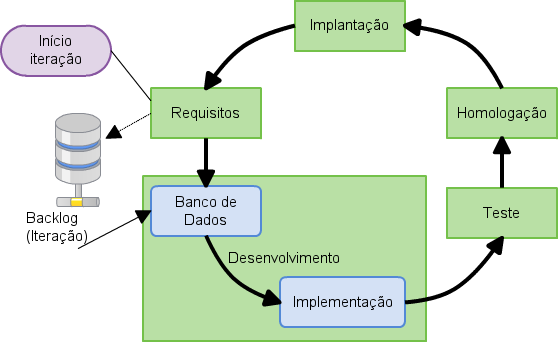
\includegraphics[scale=0.8]{figuras/ciclo_vida_solucao}
%	\caption{Ciclo de vida da solução.}
%\end{figure}

A organização do ciclo de vida foi baseada na metodologia ágil \textit{Scrum}. A idéia básica desta organização é: definir o \textit{backlog} de um ciclo (\textit{backlog} da iteração) junto com o cliente, e então ir "consumindo" esse \textit{backlog} ao longo de todo o ciclo da solução, onde cada item do \textit{backlog} definido deverá caminhar sequencialmente pelas fases do ciclo de vida. Uma vez que todo o \textit{backlog} foi "consumido" pelo ciclo de vida, temos o fim de um ciclo ou iteração. Ao completar uma iteração, um novo \textit{backlog} é definido com o cliente, e então um novo ciclo se inicia. Esse fluxo se repete até que o sistema chegue ao nível desejado pelo o cliente. As fases do ciclo de vida são descritas da seguinte forma:

\begin{itemize}
\item \textbf{Requisitos}: Priorizar as funcionalidades a serem desenvolvidas em um ciclo (\textit{backlog} da iteração), de acordo com os requisitos levantados junto com o cliente.
\item \textbf{Desenvolvimento}: Dividida pelas sub-fases de Banco de dados e de Implementação, esta fase tem o objetivo de realizar a construção do sistema. A sub-fase de Banco de dados tem o objetivo de construir o modelo de dados, tanto lógico quanto físico. Já a sub-fase de Implementação objetiva implementar de fato o sistema, baseado no modelo de dados construído.
\item \textbf{Teste}: Realizar os testes, tanto a nível de páginas da aplicação, quanto a nível de código, objetivando corrigir erros encontrados.
\item \textbf{Homologação}: Homologar a aplicação junto ao cliente, e realizar a construção de materiais de apoio ao usuário, como guias, manuais e etc. Caso não seja homologada pelo cliente, volta-se a fase do ciclo de vida necessária para realizar as correções, e a partir dali continua seguindo o ciclo sequencialmente, passando por todas as etapas sub-sequentes novamente.
\item \textbf{Implantação}: Planejar e realizar a migração do sistema para a produção.
\end{itemize}


Ao todo 18 atividades, 14 guias e 5 funcionalidades compõem a solução, onde os guias e as funcionalidades são suportes a execução de uma determinada atividade. A figura 5 ilustra a solução elaborada, agrupando todas as atividades, as funcionalidades e os guias, pelas fases do ciclo de vida. A cor azul representa as atividades, e a cor amarela representa os guias e as funcionalidades. Um guia ou uma funcionalidade identado dentro de uma atividade significa que ele é um suporte a atividade em questão.
\clearpage

\begin{landscape}
\vspace*{\fill}
\begin{figure}[!htb]
	\centering
		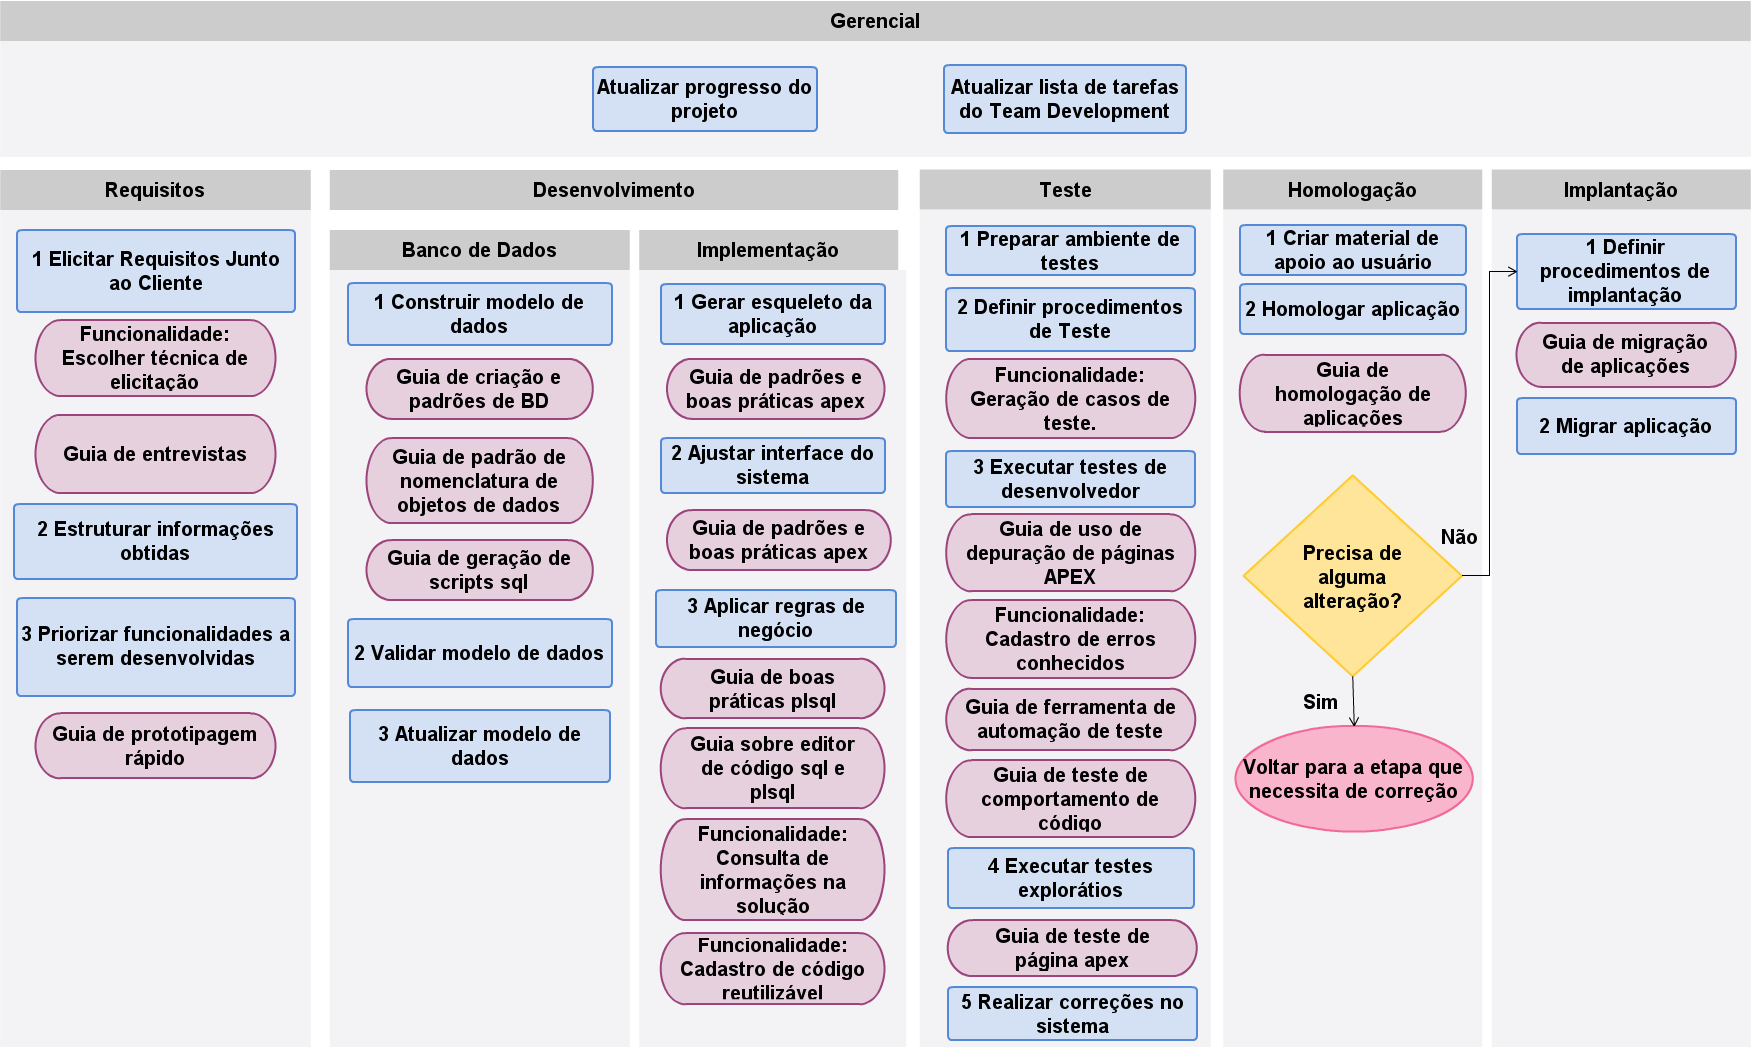
\includegraphics[scale=0.4]{figuras/fluxograma_solucao}
	\caption{Conjunto de atividades, guias e funcionalidades, por fase do ciclo de vida}
\end{figure}
\end{landscape}

Nesta solução, o ponto de decisão na fase de homologação, representado pelo losango verde, indica se a execução do fluxo irá continuar ou se irá voltar a alguma atividade dentro de uma determinada fase. Esta atividade dependerá das solicitações feitas pelo cliente durante a atividade de "Homologar aplicação".

As atividades, guias e funcionalidades são descritas brevemente da seguinte forma:

\begin{itemize}
\item \textbf{Requisitos}
\begin{enumerate}
\item \textit{Elicitar Requisitos Junto ao Cliente:} Identificar os requisitos funcionais e não funcionais da aplicação, junto com o cliente.
\item \textit{Funcionalidade - Escolher técnica de elicitação:} Funcionalidade para ajudar o desenvolvedor a escolher uma técnica de elicitação para o levantamento de requisitos junto com o cliente. Algumas técnicas já estarão pré-cadastradas, e uma delas será sugerida ao usuário com base nas respostas de algumas perguntas.
\begin{enumerate}
\item \textit{Guia de entrevistas:} Guia de como elaborar perguntas para uma entrevista com o cliente. Este guia será útil somente para quem for utilizar a entrevista como técnica de elicitação.
\end{enumerate}
\item \textit{Estruturar informações obtidas:} Transformar as informações obtidas na entrevista em requisitos, e armazená-los em documento.
\item \textit{Priorizar funcionalidades a serem desenvolvidas:} Priorizar as funcionalidades a serem desenvolvidas dentro de um ciclo da solução.
\begin{enumerate}
\item \textit{Guia de prototipagem rápido:} Guia de como realizar uma prototipagem rápida das telas de uma aplicação.
\end{enumerate}
\end{enumerate}
\item \textbf{Desenvolvimento}
\begin{itemize}
\item \textbf{Banco de Dados}
\begin{enumerate}
\item \textit{Construir modelo de dados:} Realizar a construção do modelo de dados lógico e físico.
\begin{enumerate}
\item \textit{Guia de criação e padrões de BD:} Guia com dicas de como realizar a modelagem conceitual (MER) e lógica (ML) do banco de dados da aplicação, utilizando a ferramenta Oracle Data Modeler. Utiliza o guia de padrão de nomenclatura de objetos de dados, no auxílio da construção dos modelos.
\begin{enumerate}
\item \textit{Guia de padrão de nomenclatura de objetos de dados:} Guia contendo os padrões de nomenclatura usados no órgão para diversos objetos do banco de dados, como tabelas, sequências, gatilhos e \textit{views}.
\end{enumerate}
\item \textit{Guia de geração de scripts sql:} Guia de como gerar os \textit{scripts} para a construção do modelo físico, a partir do modelo lógico, elaborado na ferramenta Oracle Data Modeler.
\end{enumerate}
\item \textit{Validar modelo de dados:} Realizar a validação do modelo de dados lógico e/ou físico, conforme a necessidade, com a área técnica responsável.
\item \textit{Atualizar modelo de dados:} Atualizar o modelo de dados, conforme as validações realizadas com a área técnica.
\end{enumerate}
\item \textbf{Implementação}
\begin{enumerate}
\item \textit{Gerar esqueleto da aplicação:} Gerar o esqueleto da aplicação usando a funcionalidade \textit{defaults} de interface de usuário do APEX.
\item \textit{Ajustar interface do sistema:} Refinar a interface da aplicação conforme as necessidades de usabilidade da mesma.
\item \textit{Guia de boas práticas APEX:} Guia para auxiliar a criação da aplicação, usando boas práticas em APEX.
\item \textit{Aplicar regras de negócio:} Implementar as regras de negócio da aplicação.
\begin{enumerate}
\item \textit{Guia de boas práticas plsql:} Guia para auxiliar a construção de código em PL/SQL.
\item \textit{Guia sobre editor de código sql e plsql:} Guia para auxiliar o uso do editor de código para a escrita de códigos SQL e PL/SQL.
\item \textit{Funcionalidade - Cadastro de código reutilizável:} Funcionalidade para permitir que o desenvolvedor possa cadastrar códigos que ele julgue que possam ser reutilizáveis.
\end{enumerate}
\item \textit{Funcionalidade - Consulta de informações na solução:} Consulta conveniente das informações da solução, de forma a permitir um acesso mais rápido a um determinado guia ou funcionalidade. O usuário também pode cadastrar suas anotações. A idéia é semelhante a de uma \textit{Wiki}.
\end{enumerate}
\end{itemize}
\item \textbf{Teste}
\begin{enumerate}
\item \textit{Preparar ambiente de testes:} Realizar os preparativos necessários ao ambiente para a realização dos testes da aplicação. Ex: Criar massa de dados, limpar dados existentes, criar um novo espaço de trabalho APEX, e etc.
\item \textit{Definir procedimentos de teste:} Definir um conjunto de etapas a serem realizadas nos testes.
\begin{enumerate}
\item \textit{Funcionalidade - Geração de casos de teste:} Funcionalidade que auxilie os testes do desenvolvedor, oferecendo diferentes valores que o usuário pode inserir nos diferentes componentes da interface, de forma a testar várias possibilidades diferentes.
\end{enumerate}
\item \textit{Executar testes de desenvolvedor:} Executar os testes planejados.
\begin{enumerate}
\item \textit{Guia de uso de depuração de páginas APEX:} Guia explicando como usar a funcionalidade de depurar existente no APEX, para encontrar erros na aplicação.
\item \textit{Funcionalidade - Cadastro de erros conhecidos:} Funcionalidade que permita que o desenvolvedor possa cadastrar os erros que for encontrando, de forma a montar uma espécie de base de conhecimento de erros.
\item \textit{Guia de ferramenta de automação de teste:} Guia que auxilie o desenvolvedor a criar \textit{scripts} simples de automação de ações no navegador, de forma a criar testes automatizados.
\item \textit{Guia de teste de comportamento de código:} Guia que auxilie o desenvolvedor a testar, dentro do possível, e realizar a depuração de códigos em PL/SQL.
\end{enumerate}
\item \textit{Executar testes exploratórios:} Navegar na aplicação, sem um prévio planejamento, em busca de erros.
\begin{enumerate}
\item \textit{Guia de teste de página APEX:} Guia com dicas de como realizar os testes exploratórios.
\end{enumerate}
\item \textit{Realizar correções no sistema:} Realizar as correções e ajustes necessários ao sistema.
\end{enumerate}
\item \textbf{Homologação}
\begin{enumerate}
\item \textit{Criar material de apoio ao usuário:} Criar um guia que auxilie o usuário a usar a aplicação.
\item \textit{Homologar aplicação:} Realizar a homologação da aplicação, junto ao cliente.
\begin{enumerate}
\item \textit{Guia de homologação de aplicações:} Guia com dicas de como realizar a homologação junto ao cliente.
\end{enumerate}
\end{enumerate}
\item \textbf{Implantação}
\begin{enumerate}
\item \textit{Definir procedimentos de implantação:} Definir as etapas necessárias para colocar a aplicação em produção.
\begin{enumerate}
\item \textit{Guia de migração de aplicações:} Guia com dicas do que se preocupar ao realizar a migração de uma aplicação APEX.
\end{enumerate}
\item \textit{Migrar aplicação:} Executar os procedimentos de migração definidos.
\end{enumerate}
\end{itemize}
De forma a auxiliar o desenvolvedor na gerência do desenvolvimento, uma adaptação do \textit{Kanban} foi feita, e ela pode ser visualizada na figura 6. \clearpage

\begin{landscape}
\vspace*{3cm}
\begin{figure}[!htb]
	\centering
		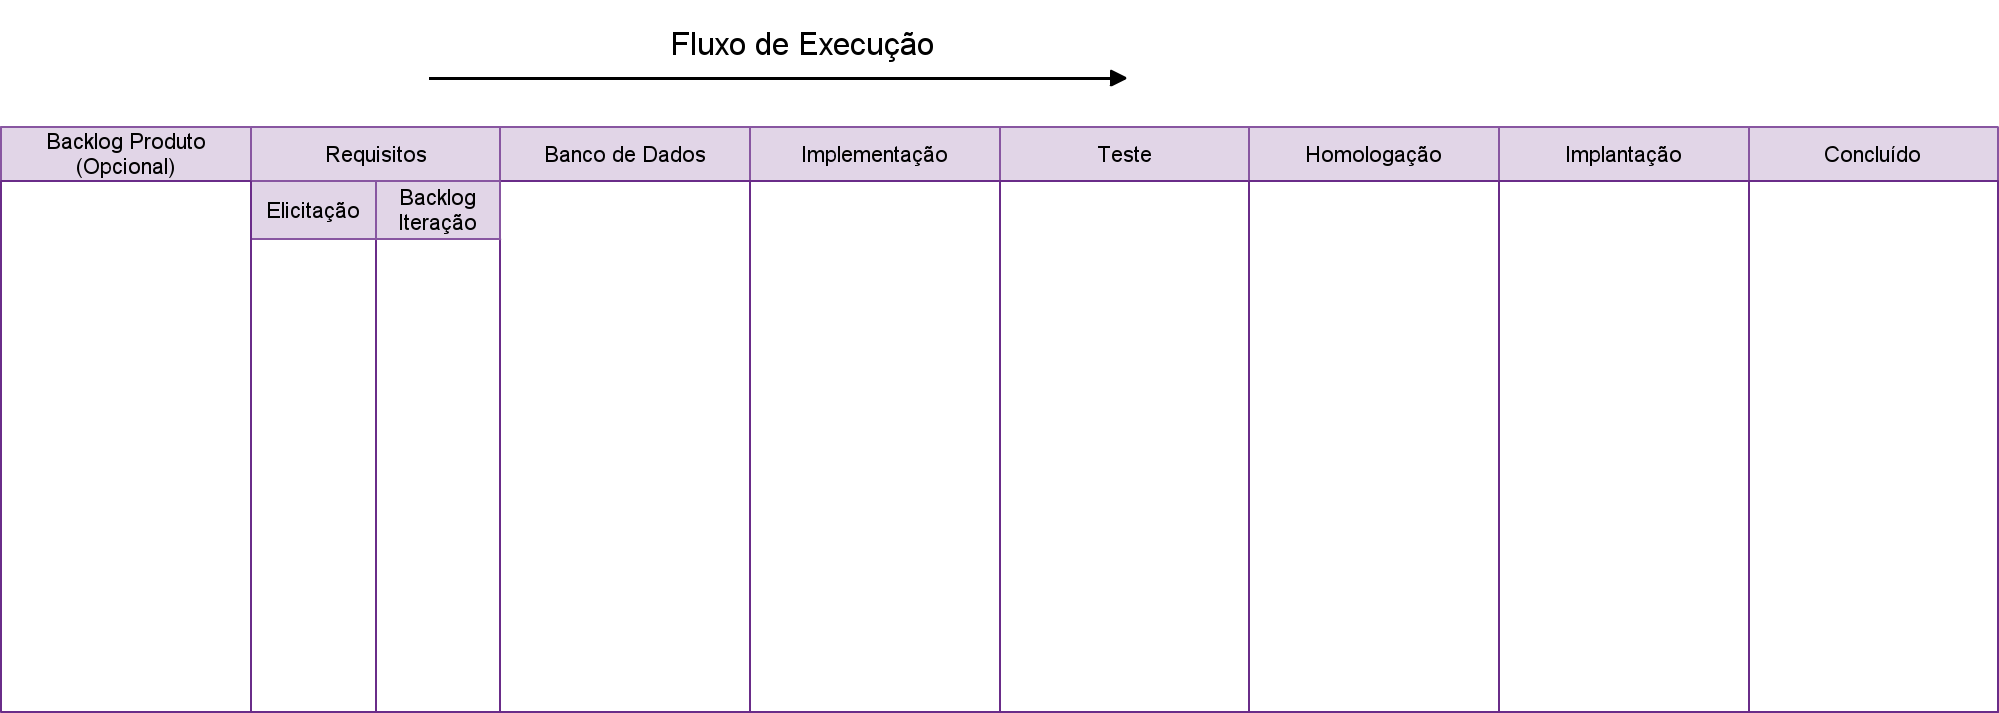
\includegraphics[scale=0.35]{figuras/kanban}
	\caption{Conjunto de atividades, guias e funcionalidades, por fase do ciclo de vida}
\end{figure}
\end{landscape}

Este \textit{Kanban} foi dividido pelas fases do ciclo de vida da solução, de forma que o desenvolvedor vai posicionando os itens do \textit{backlog} definido, de acordo com a etapa em que se encontram dentro do ciclo de vida. A ideia é que o \textit{backlog} da iteração gerado seja em pequenas unidades de funcionalidades, de forma a facilitar o gerenciamento e acompanhamento pelo desenvolvedor. Ao terminar um conjunto destas unidades de funcionalidade, o desenvolvedor consegue gerar um entregável ao cliente. Observa-se que a divisão \textit{Backlog} Produto é opcional, já que pode ser da preferência do cliente e do desenvolvedor levantar o \textit{backlog} do produto. Porém, neste caso, o fluxo de execução do \textit{Kanban} obriga a seleção e priorização de um \textit{backlog} da iteração, conforme a divisão de Requisitos.

\chapter[Capítulo 6 – Cronograma de Execução]{Capítulo 6 – Cronograma de Execução}

\section{\textit{Considerações Iniciais do Capítulo}}

--falar sobre considerações iniciais--

\section{\textit{Cronograma Elaborado}}

\section{\textit{Considerações Finais}}